\chapter{Phenomenology of particle physics and experimental status}
\label{ch:pheno}

The idea that our universe is composed of very small and indivisible particles is not new, and has its origins in various cultures.
The word \emph{atom}, which is derived from the Greek word \emph{atomos}, also means \emph{unbreakable}.
Currently, the theory that brings together our understanding of matter, the \emph{elementary particles}, and its interactions, called \emph{forces}, is called the Standard Model of Particle Physics (SM).
This model provides a unified picture where the forces between particles are themselves described by the exchange of particles.
Remarkably, the Standard Model succeeds in describing most current experimental data and represents one of the triumph of modern physics.

Nevertheless, some questions are still open, for which the SM does not provide answers, as the matter/antimatter asymmetry of the universe, the dark matter nature and the origin of neutrino masses.
In order to account for these three observational discrepancies, new physics models have to be investigated.
If a satisfactory theory beyond the Standard Model emerges, bringing an explanation to these open questions, it could greatly impact our comprehension of the fundamental mechanisms of the Universe.
In particular, the third one, concerning the mass of neutrinos, is the one which ultimately motivated this PhD, and is therefore particularly described in this chapter.
It could also have an impact on the comprehension of matter/antimatter asymmetry origin.

\section{The Standard Model of particle physics}


The Standard Model of particle physics describes the strong, weak and electromagnetic interactions, gauged by the symmetry group $SU(3)_{C}\times SU(2)_{L}\times U(1)_{Y}$, where $C$ represents the colour, $L$ the left-handed chirality and $Y$ the hypercharge.
The SM gauge bosons (the $8$ gluons, $Z_{0}$, $W^{\pm}$ and the photon) mediate these interactions.
The scalar Higgs field is at the origin of electroweak symmetry breaking (i.e. $SU(2)_{L}\times U(1)_{Y} \rightarrow U(1)_{em}$), and is responsible for giving masses to elementary particles.

\subsection{Particle content}

The particle content is presented in Fig.~\ref{fig:SM_chart}.
\begin{figure}[h!]
  \centering
  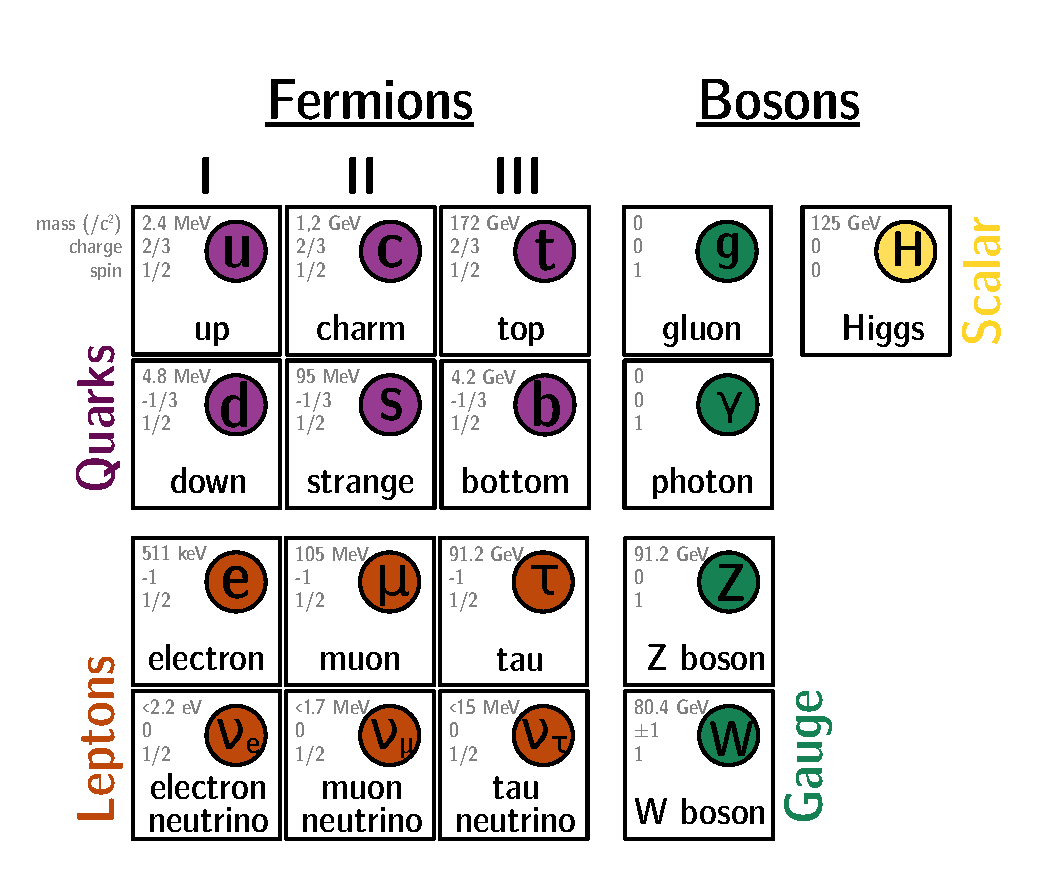
\includegraphics[width=1\textwidth]{neutrinophysics/fig_neutrinophysics/SM_chart.pdf}
  \caption{The Standard Model of elementary particles.
    \label{fig:SM_chart}}
\end{figure}

\subsubsection*{Fermions}

Fermions are particles with half-integer spins, obeying to the Pauli exclusion principle.
The properties of the $12$ fermions of the Standard Model allow to classify them into categories, according to the forces to which they are sensitive.
All fermions experience the weak force, while only $9$ of them participate in the electromagnetic interaction of QED, the neutrinos being electrically neutral.
Only quarks feel the strong force, as they are the only ones carrying the QCD charge.
The SM fermions are further classified in three generations.

To construct the electroweak $SU(2)_L \times U(1)_Y$ theory, the fermions field can be represented through their chirality properties.
For one given generation, the left-handed chiral components of the fermion fields are grouped into $SU(2)$ doublets
\begin{equation}
  L_{L}=
  \begin{pmatrix}
    \nu_{L} \\
    l_{L}
  \end{pmatrix}
  \qquad and \qquad
  q_{L}=
 \begin{pmatrix}
    u_{L} \\
    d_{L}
 \end{pmatrix}
 \,,
 \label{eq:fermion_doublet}
\end{equation}
where $L_L$ stands for the leptons and $q_L$ for the quarks.
In the SM, neutrinos are assumed to have only left-handed components, since they are described as mass-less.
The right-handed components of the other fermions are $SU(2)$ singlets, $e_R$, $u_R$ and $d_R$.
The generalisation for three generations is not presented in this chapter.

\subsubsection*{Bosons}

Bosons are particles with integer spins, described by the Bose-Einstein statistics.
The elementary bosons of the SM are also called gauge bosons have a spin $1$, and mediate the interaction between elementary particles.
The Higgs bosons, with a spin $0$, is a scalar boson.

\subsection{Where the Standard Model ends}


An ultimate Model of particle physics should theoretically predict and explain all particle masses and interactions, with few free parameters.
Despite the success of the Standard Model in the explanation of particle behaviours, unanswered questions remain.
\begin{itemize}
\item Matter/antimatter asymmetry\\
  The beginning of the Universe should have produced the same quantity of matter and antimatter, simply because nor matter nor antimatter should be advantaged over the other.
  Nevertheless, from experimental evidences, we know that the former dominates over the latter, known as Baryonic Asymmetry of the Universe (BAU).
  The amount of charge-parity (CP) violation observed in the quark sector being not sufficient to explain this asymmetry, the SM fails to explain this unbalance.
\item Dark matter\\
  The known matter described by the SM represents only $5$\% of the Universe composition.
  Another $27$\% represents matter existing in a \emph{non-luminous} form, called Dark Matter (DM), for which the Standard Model does not provide a viable candidate.
  Such matter is colourless and electrically neutral, and can only have weak and/or gravitational interactions.
  Early evidence for the existence of DM was provided by galaxy rotation curves: relying only on \emph{luminous} matter, the velocity should decrease as $r^{-1/2}$, where $r$ is the distance to the galaxy centre.
  This is in disagreement with observation, suggesting the existence of additional matter.
  The remaining $68$\% of the universe composition is composed of dark energy, an unknown form of energy introduced, among others, to explain the accelerated expansion of the universe.
\item Neutrino masses\\
  Providing an explanation to neutrino masses, and understanding their smallness compared to other fermions, is an important question in modern particle physics.
  First proposed by Fermi in $1933$~\cite{art:fermi_1933}, neutrinos were believed to be mass-less, and in its original formulation, the SM included no neutrino mass term.
  Neutrino oscillations, which are confirmed by a plethora of experiments, provided evidence for neutrino masses.
  Given their unique neutral character, neutrinos can be either Dirac (particles and anti-particles are distinct) or Majorana (particles are their own anti-particles) fermions.
  Looking for neutrinoless beta decays is one of the preferred ways to probe the Majorana nature of neutrinos.
\end{itemize}
This is a non-exhaustive list, and other tensions exist between theory and observation, such as the anomalous magnetic moment of the muon, or the flavour universality violation in B and D meson decays.


\section{Going beyond the Standard Model with neutrinos}
\subsection{Neutrino flavors and oscillations}

The neutrinos are only detected through their weak interaction with matter, which defines the three neutrino flavours.
For instance, an electron neutrino $\nu_e$ is defined as the particle produced through a charged-current weak interaction with an electron.
In the same manner, the charged-current weak interaction of an electron neutrino produces an electron.

The first (and only) evidence that neutrinos are massive is the observation of neutrino oscillations, first predicted in 1957 by Pontecorvo~\cite{art:pontecorvo_1958}.
In 1998 emerged from the Super-Kamiokande experiment the confirmation for neutrino flavour changing: the deficit of muon neutrinos was inconsistent with expectations based on calculations of the atmospheric neutrino flux, suggesting that muon neutrinos oscillate with tau neutrinos~\cite{art:kamiokande_1998}.

\subsubsection*{Flavour and mass eigenstates}


The neutrino oscillation is a quantum-mechanical effect, which can be understood in terms of the relationship between the three weak interaction eigenstates, $\nu_e$, $\nu_{\mu}$ and $\nu_{\tau}$ that can be experimentally measured, and the three mass eigenstates, $\nu_1$, $\nu_2$ and $\nu_3$, that propagate in space-time.
If the neutrino mass is zero thus, in the charged lepton sector, a basis can always be defined such as the lepton mass matrix is diagonal.
However, by introducing even small masses for the neutrinos, a common basis were the two lepton mass matrix are diagonal can't be found.
The neutrino interaction and mass eigenstate are related by the $U_{PMNS}$ matrix such as
\begin{equation}
  \begin{pmatrix}
    \nu_e \\
    \nu_{\mu} \\
    \nu_{\tau}
  \end{pmatrix}
  =
  \begin{pmatrix}
    U_{e1} & U_{e2} & U_{e3} \\
    U_{\mu 1} & U_{\mu 2} & U_{\mu 3} \\
    U_{\tau 1} &  U_{\tau 2} &  U_{\tau 3} \\
  \end{pmatrix}
  \begin{pmatrix}
    \nu_1 \\
    \nu_2 \\
    \nu_3
  \end{pmatrix}
  \,,
  \label{eq:upmns}
\end{equation}
where $U_{e2}$ denotes the $\nu_2$-component of the interaction eigenstate $\nu_e$, for instance.

\subsubsection*{Oscillation probability}

Considering two-flavour neutrino $\nu_{\alpha}$ and $\nu_{\beta}$, the oscillation probability is written as
\begin{equation}
  \mathcal{P}_{\nu_{\alpha}\rightarrow \nu_{\beta}}(t)=\sin^{2}({2\theta})\sin^{2}\left({\frac{\Delta m^2}{4E}}L\right)\qquad (\nu_{\alpha}\neq\nu_{\beta})
  \label{eq:osc_proba}
\end{equation}
where $L$ is the source-detector distance, $E$ is the neutrino energy and $\theta$ is the mixing angle with a value in the interval ${0\leq\theta\leq\pi/2}$.
In the particular case of two-neutrino mixing the squared mass difference $\Delta m^2$ is defined as
\begin{equation}
\Delta m^2=\Delta m_{12}^2=m_2^2-m_1^2\,,
\end{equation}
where $m_1$ and $m_2$ are the masses of the states $\nu_1$ and $\nu_2$ defined as $m_1<m_2$ so that $\Delta m^2>0$.
The first observation coming with Eq.~\eqref{eq:osc_proba} is that if neutrino masses were not degenerated, oscillations would not be possible.
A direct consequence of this statement is that if neutrinos are mass-less, they cannot oscillate.
Then, we only need two non-zero neutrino masses for neutrino oscillation to be observed.
Therefore, a minimal model including neutrino masses only requires two RH neutrinos (considering the lightest active neutrino is mass-less).

Neutrino mixing is a quantum effect: an interaction state $\nu_{\alpha}$ is produced in a well-determined state, which is a linear combination of the three mass eigenstates.
When the neutrino propagates through space-time, these coefficient are free to evolve as long as the neutrino is not detected and therefore measured.
The neutrino is then no more determined as $\nu_{\alpha}$.
When the neutrino is detected, an eigenstate is determined in the interaction basis, corresponding to $\nu_e$, $\nu_{\mu}$ or $\nu_{\tau}$.
Thus $\nu_{\alpha}$ can be measured as another neutrino state, with the probability given in Eq.~\eqref{eq:osc_proba}.

\subsubsection*{Neutrinos mass ordering}

The sensitivity to $\Delta m^2$ of an experiment is the value of $\Delta m^2$ for which ${\Delta m^2 L/2E \sim 1}$, allowing to classify neutrino experiments.
Atmospheric neutrinos are created by the interaction between the cosmic rays and the nuclei in the earth's atmosphere: protons of the cosmic rays interact with atmospheric nuclei, mostly producing pions.
Pions mainly decay into muons and muon neutrinos in the energy range of $[0.5-10^2]$~GeV.
Atmospheric neutrino experiments, with a source-detector distance about $10^4$~km, are then sensitive to $\Delta m^2\sim 10^{-4}$~eV$^2$, above the order of magnitude of $\Delta m^2_{32}$ , which allow to rename $\Delta m^2_{32} = \Delta m^2_{atm}$.
In nuclear fusion processes, protons are transformed into neutrons through a weak process, producing electron neutrinos with an energy about $[0.2-15]$~MeV.
Since the sun-earth distance is about $1.5\times 10^{11}$~km, solar neutrino experiments are sensitive to $\Delta m^2 \sim 10^{-12}$~eV$^2$.
Comparing this sensitivity with $\Delta m^2_{12}$, one can write $\Delta m^2_{12} = \Delta m^2_{sol}$.
The study of neutrino mixing allows us to have access to precise values of squared mass differences $\Delta m^2_{sol}$ and $\Delta m^2_{atm}$.

Thanks to matter effects in the Sun, we know that $\Delta m^2_{sol}>0$.
Since $\Delta m^2_{atm}$ is essentially measured via neutrino oscillations in vacuum, which exclusively depend on its absolute value, its sign is unknown at the moment.
Therefore, the neutrino masses can be ordered in two ways: normal ordering (NO) if $\Delta m^2_{atm}>0$ and inverted ordering (IO) if $\Delta m^2_{atm}>0$.
Both orderings are presented in Fig.~\ref{fig:IO_NO}
Indirect constraints may come from the observation of the neutrinoless double beta decay or from cosmological bounds on the sum of the neutrino masses.
\begin{figure}[h!]
  \centering
  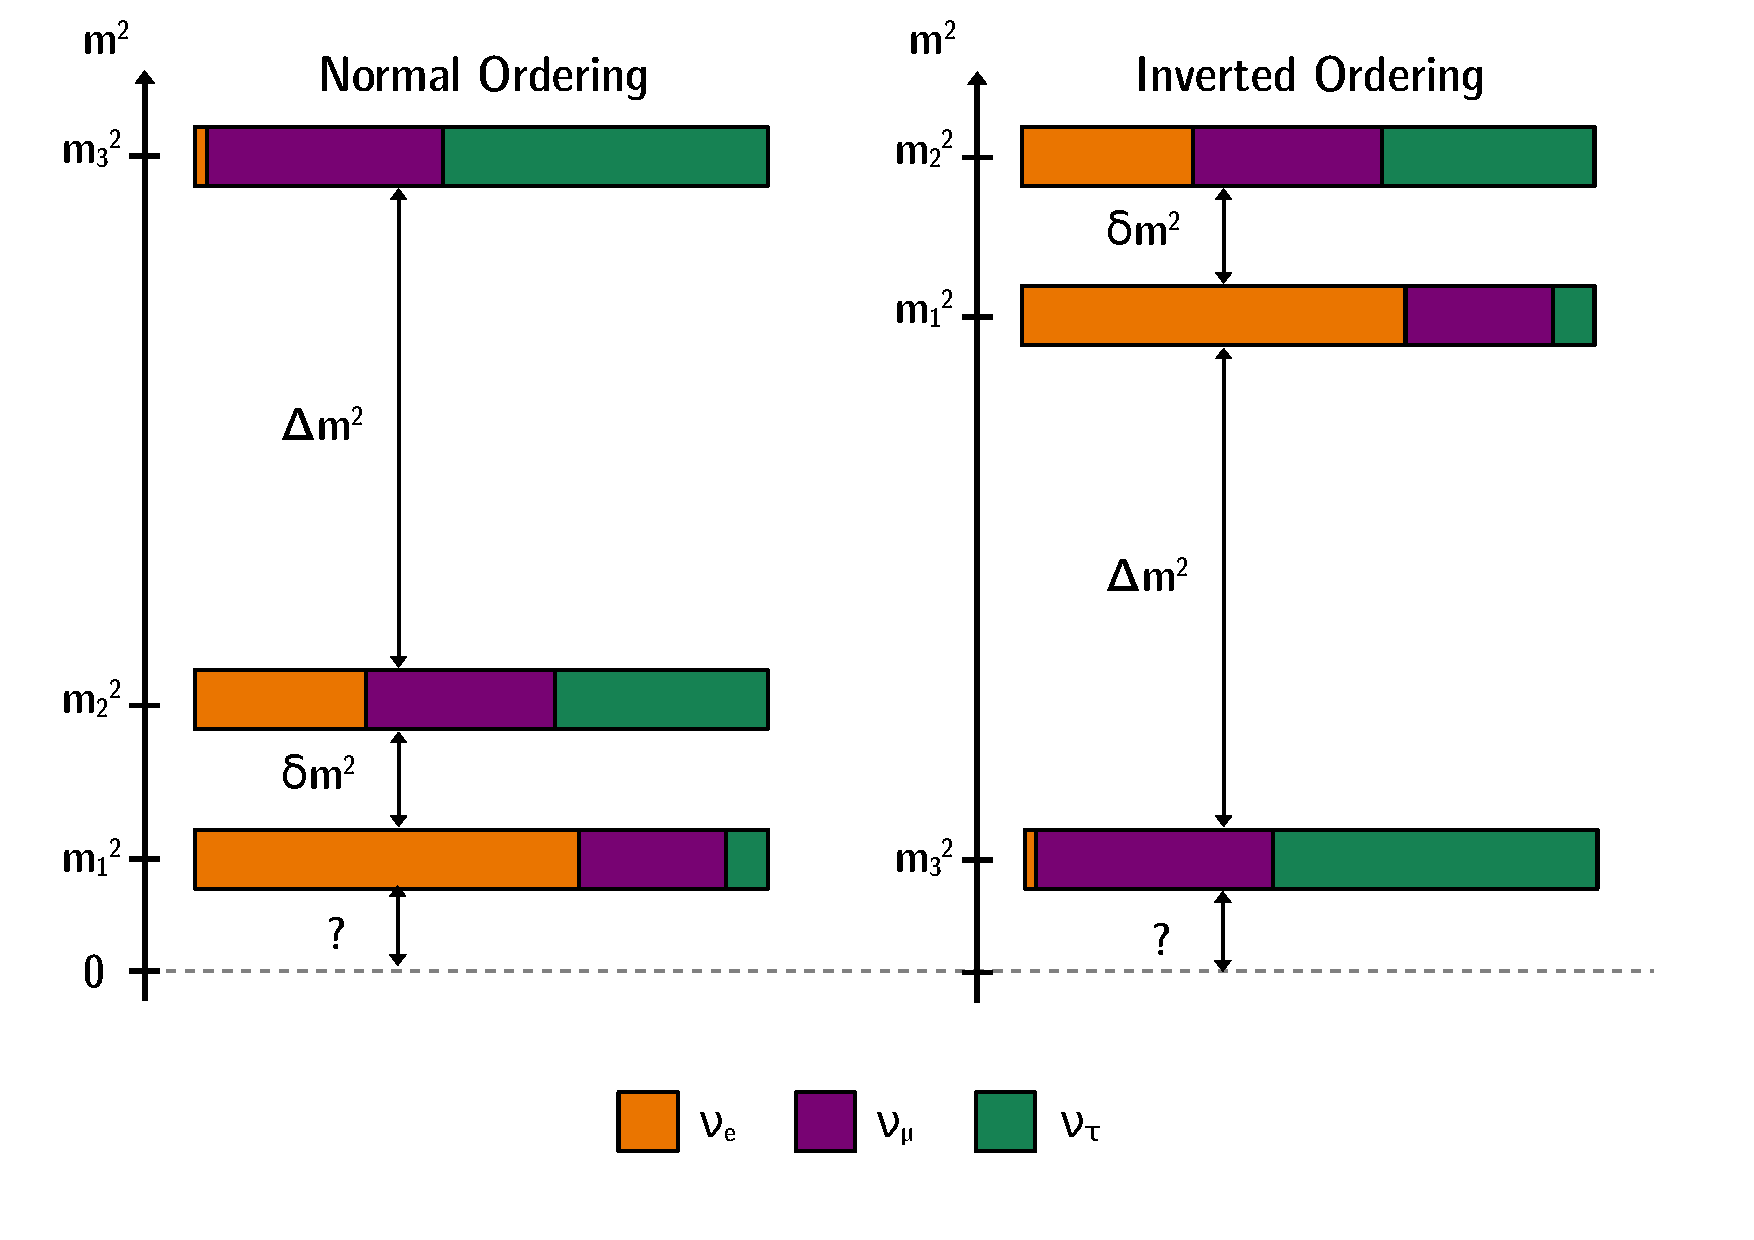
\includegraphics[width=1\textwidth]{neutrinophysics/fig_neutrinophysics/IO_NO.pdf}
  \caption{Graphic view of the probability of finding one of the flavor eigenstates if the neutrino is in a certain mass eigenstate.
    Normal and inverted orderings are presented.
    ${\delta m^2=m_2^2-m_1^2}$ and ${\Delta m^2=m_3^2-(m_1^2+m_2^2)/2}$.
    \label{fig:IO_NO}}
\end{figure}

\subsubsection*{Oscillation data}

The leptonic mixing matrix defined in Eq.~\eqref{eq:upmns} can be parameterised as
\begin{equation}
  U_{PMNS}=
  \begin{pmatrix}
    c_{12}c_{13} & s_{12}c_{13} & s_{13}e^{-i\delta_{CP}} \\
    -s_{12}c_{23}-c_{12}s_{23}s_{13}e^{i\delta_{CP}} & c_{12}c_{23}-s_{12}s_{23}s_{13}e^{i\delta_{CP}} & s_{23}c_{13} \\
    s_{12}s_{23}-c_{12}c_{23}s_{13}e^{i\delta_{CP}} &  -c_{12}s_{23}-s_{12}c_{23}s_{13}e^{i\delta_{CP}} &  c_{23}c_{13} \\
  \end{pmatrix}
  \label{eq:upmns_detail}
\end{equation}
where $c_{ij}=\cos{\theta_{ij}}$, $s_{ij}=\sin{\theta_{ij}}$ and $\delta_{CP}$ is the Dirac CP violating phase.
Tab.~\ref{tab:best_fit} sums up the latest best fit values of $U_{PMNS}$ parameters~\cite{art:Capozzi_2017}.
\begin{table}[h]
  \centering
  \begin{tabular}{|c|c|c|}
    \hline
    Parameter & Hierarchy & Best fit \\
    \hline\hline
    $\Delta m^{2}_{12}$ ($10^{-5}$eV$^{2}$) & NO or IO & $7.37$ \\
    \hline
    $\sin^{2}\theta_{12}$ ($10^{-1}$) & NO or IO & $2.97$ \\
    \hline
    $\Delta m^2$ ($10^{-3}$eV$^{2}$) & NO & $2.52$ \\
    $\Delta m^2$ ($10^{-3}$eV$^{2}$) & IO & $2.50$ \\
    \hline
    $\sin^{2}\theta_{13}$ ($10^{-2}$) & NO & $2.15$ \\
    $\sin^{2}\theta_{13}$ ($10^{-2}$) & IO & $2.15$ \\
    \hline
    $\sin^{2}\theta_{23}$ ($10^{-1}$) & NO & $4.22$ \\
    $\sin^{2}\theta_{23}$ ($10^{-1}$) & IO & $5.90$ \\
    \hline
    $\delta_{CP}/\pi$ & NO & $1.40$ \\
    $\delta_{CP}/\pi$ & IO & $1.30$ \\
    \hline
  \end{tabular}
  \caption{Best fit values of neutrino oscillation parameters, for inverted and normal orderings (IO and NO, respectively)~\cite{art:Capozzi_2017}.
    ${\Delta m^{2}=m_3^2-(m_1^2+m_2^2)/2}$ with $+\Delta m$ for IO.
    The CP violating phase is taken in the interval $0\leq\delta_{CP}/\pi\leq2$.
    \label{tab:best_fit}}
\end{table}

Fig.~\ref{fig:ckm_pmns} pictures the relative different contributions of quark and neutrino matrix elements.
Unlike the CKM matrix for the quark sector, the neutrino mixing angles are found to be large.
This can be explained by the different forces to which quarks and neutrinos are sensitive.
Indeed, whenever the interaction eigenstates are not equal to the mass eigenstates, particles can experience oscillations.
Experimentally, whether or not these oscillations are observable depends on the interactions of the particles.
Quarks interact significantly with their environment, meaning they are often measured and thus determined in a given interaction state.
Therefore, quark oscillations exist but are highly reduced.
On the other hand, neutrinos interact very little when they propagate, thus their oscillations are experimentally measurable.
\begin{figure}[h]
  \centering
  \begin{subfigure}[t]{0.48\textwidth}
    \centering
    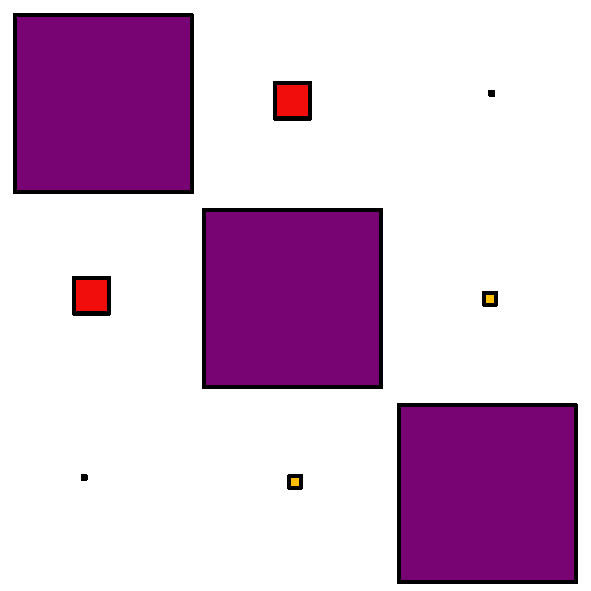
\includegraphics[height=0.7\textwidth]{neutrinophysics/fig_neutrinophysics/ckm_draw.pdf}
    \captionsetup{justification=justified}
    \caption{CKM matrix.
      \label{subfig:ckm}}
  \end{subfigure}
  \hfill
  \begin{subfigure}[t]{0.48\textwidth}
    \centering
    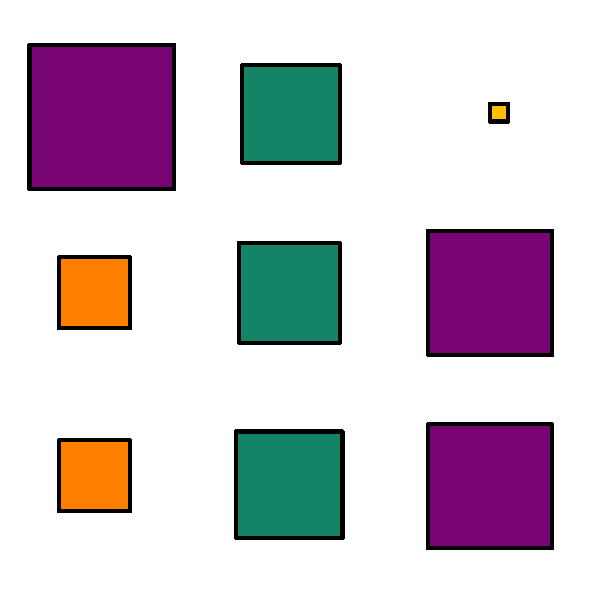
\includegraphics[height=0.7\textwidth]{neutrinophysics/fig_neutrinophysics/upmns_draw.pdf}
    \captionsetup{justification=justified}
    \caption{PMNS matrix.
      \label{subfig:pmns}}
  \end{subfigure}
  \caption{Comparison between the relative contributions of quark and neutrino matrix elements.
    The square areas stand for the square of the corresponding matrix element.
    \label{fig:ckm_pmns}
  }
\end{figure}


\subsection{Neutrino masses and nature}


As neutrinos are neutral particles, several mass terms can be introduced in the SM Lagrangian, depending on their nature.

\subsubsection{Neutrino Dirac masses}
\label{subsec:dirac_mass}

In the SM, fermions are Dirac particles, meaning particles and anti-particles are different.
Their masses arise with the Higgs mechanism, through the coupling of left- and right-handed fields with the Higgs doublet.
One can imagine the same mechanism arises for neutrinos.

In the SM, only left handed leptons participate in the charged weak interaction.
As it is the only force through which neutrinos interact, only the left-handed component is described in the SM for neutrinos.
Then, adding a Dirac term in the Lagrangian comes with introducing a right-handed chiral neutrino field, so-called sterile neutrino.
They are named that way in order to distinguish them from known left-handed active neutrinos.

\subsubsection*{Dirac spinors}

In the Standard Model, fermions are described by Dirac quantised fields $\psi(x)$, 4-component spinors which are a solution of the Dirac equation,
\begin{equation}
  (i\slashed\partial-m)\psi(x)=0\,,
  \label{eq:dirac}
\end{equation}
with $m$ the mass of charged leptons.
$\slashed\partial\equiv \gamma^{\mu}\partial_{\mu}$ where there is an implied summation over the values of the twice-repeated index $\mu=0,1,2,3$, and $\partial_{\mu}$ is the $4$-gradient.
We can describe a Dirac field in term of chiral fields as
\begin{equation}
  \psi = \psi_R + \psi_L\,,
  \label{eq:chiral}
\end{equation}
with $\psi_R$ and $\psi_L$ the eigenvectors of the $\gamma^{5}$ matrix, also called the chirality projector.
$\psi_R$ and $\psi_L$ are called Weyl spinors.
Then the Lagrangian for a free fermion field is written as
\begin{equation}
\mathcal{L} = (\overline{\psi_R} + \overline{\psi_L})(i\overleftrightarrow{\slashed{\partial}}-m)(\psi_R + \psi_L)\,.
\end{equation}
It results from Eqs.~\eqref{eq:dirac} and \eqref{eq:chiral} that $\psi_R$ and $\psi_L$ have independent kinetic terms, but coupled mass terms:
\begin{align}
i\gamma^{\mu}\partial_{\mu}\psi_L& = m\psi_R\,,\label{eq:psi_L}\\
i\gamma^{\mu}\partial_{\mu}\psi_R& = m\psi_L\,\label{eq:psi_R}\,.
\end{align}
Consequently, the two chiral component fields are independent only if $m = 0$.
%% \subsection{Bosons}
%% \subsection{Fermions}
%% \subsection{$\twonu$ decay}

\subsubsection*{Dirac mass term}

Charged leptons are massive in the SM with the Dirac mass term in the Lagrangian:
\begin{equation}
\mathcal{L}^{l}_{Y} = -\frac{v}{\sqrt{2}}\,\overline{l}^{\,'}_{L}\,Y^{\,'l}\,l^{\,'}_{R} + h.c.\,,
\end{equation}
where $Y^{\,'l}$ is the Yukawa matrix for charged leptons, $v$ is the vacuum expectation value (vev) for the Higgs field, and primed fields refer to the weak interaction basis.
In the SM Lagrangian, there is no mass term for neutrinos, and the lepton Yukawa couplings can be diagonalised without leading to flavour violation in charged lepton currents.
Thus the lepton flavour is conserved in the SM.

In the Standard Model, neutrinos only undergo weak interactions.
But weak interactions are described by the $SU(2)_L$ group, whose elements act only on left-handed chiral components of the fermion fields.
So weak interaction ``see'' only the LH components of fields.
If one goes beyond the SM, one can add a right handed neutrino $\nu_R$, singlet under all gauge interactions ($SU(3)_{C}\times SU(2)_{L}\times U(1)_{Y}$ gauge groups).
In this case, and as occurred for the quark and charged lepton sectors, neutrino masses can be generated by the Higgs mechanism, with a Dirac mass term:
\begin{equation}
\mathcal{L}^{\nu}_{Y} = -\frac{v}{\sqrt{2}}\,\overline{\nu}^{\,'}_{L}\,Y^{\,'\nu}\,\nu^{\,'}_{R} + h.c.\,.
\label{eq:dirac_mass_term}
\end{equation}
Thus to have a Dirac mass term in the Lagrangian, we need to introduce right handed neutrinos $\nu_R$, called sterile neutrinos, because they do not interact through weak interaction, unlike active neutrinos.
If neutrinos and leptons are both massive, one cannot have $Y^\nu$ and $Y^l$ simultaneously diagonal.
Then the leptonic charged currents are not diagonal anymore, leading to lepton flavour violation.
That leads to new processes including neutrino oscillations.

It is important to notice that for Dirac neutrinos, and even if their masses are described by the same mechanism responsible for all other SM fermion masses, the corresponding Yukawa couplings are extremely tiny, many orders of magnitude below $Y^l$ and $Y^q$ (the Yukawa matrix for quarks).

\subsubsection{Neutrino Majorana masses}
\label{subsec:maj_mass}

\subsubsection*{Majorana neutrinos}

As we have seen in the previous sub-section, $4$-component Dirac spinors are used to describe fermion fields.
As Eqs.~\eqref{eq:psi_L} and~\eqref{eq:psi_R} are coupled, we could derive one simple expression if we find a link between $\psi_R$ and $\psi_L$.
In the $1930$'s Ettore Majorana suggested such a link by writing $\psi_R = C\overline{\psi}_L^{\,T}$, where $C$ is the charge conjugation matrix and $\overline{\psi} = \gamma^0\psi$.
Therefore $C\overline{\psi}_L^{\,T}$ is right-handed.
We thus have the Majorana condition for fields
\begin{equation}
  \psi=C\overline{\psi}^{\,T}\,,
  \label{eq:maj_cond}
\end{equation}
since we have the chiral description for fermion fields in Eq.~\eqref{eq:chiral}.
With this condition, fermion fields are now described by a $2$-component spinor.
Thus a Majorana field has half the number of degree of freedom of a Dirac field.
As $C\overline{\psi}_L^{\,T}$ is equivalent to $\psi_{L}^{C}$~\cite{book:giunti}, the Majorana condition in Eq.~\eqref{eq:maj_cond} can be written as $\psi = \psi^C$.
This further implies that a Majorana particle is its own antiparticle.
Therefore, Majorana and Dirac particles are fundamentally different particles.

\subsubsection*{Majorana mass term}

An effective field theory (EFT) is an ``approximation'' of a more general theory.
It is used when a physical process is studied at such low energies (or long distances) that we cannot probe the underlying phenomenon that occurs (one says that the heavy fields at the origin of such
interactions are ``integrated out'').
Fermi first described the weak interaction of beta decay with an EFT, when only leptons and hadrons were known.
This so-called Fermi theory describes a contact interaction between $4$ SM fields.
In a more general manner, an effective Lagrangian, which generalises the SM one, has an infinite number of terms as
\begin{equation}
  \mathcal{L}_{eff}=\mathcal{L}_{SM}+\sum_{d}\frac{1}{\Lambda^{d-4}}C^{d}O^{d}\,,
\end{equation}
with $d>4$.
$C$ represents the couplings at the effective vertex, and $O$ is an effective non-renormalisable operator with a dimension above $4$, which contains only SM fields.
For the neutrino case, we want to write a mass term involving only SM fields, that means with the only left-handed neutrino field $\nu_L$.
The operator with the lowest dimension - which respects the SM symmetries - to describe neutrino masses in the SM (without RH neutrinos) is a dimension-$5$ operator, called the Weinberg operator, which can be represented as in Fig.~\ref{fig:weinberg_diagram} and defined as
\begin{equation}
  \mathcal{L}_5 = \frac{1}{2}\frac{g^{eff}}{\mathcal{M}}(\overline{L}_{L}^{\,c}\sigma^{2}\phi)(\phi^{\,T}\sigma^{2}L_L)+h.c.\,,
  \label{eq:lag_5}
\end{equation}
where $g^{eff}$ is a dimensionless coefficient corresponding to a new effective coupling and $\sigma$ the Pauli matrices.
$L_L$ is defined by Eq.~\eqref{eq:fermion_doublet} and $\phi$ represents the Higgs field.
In Eq.~\eqref{eq:lag_5}, the coefficient $C$ is here identified with $g^{eff}/2$, and $O$ is represented by the [LH][LH] operator.
This Lagrangian respects all the SM symmetries, except for the total lepton number conservation.
After the electroweak symmetry breaking, the following Lagrangian stands for the neutrino fields
\begin{equation}
  \mathcal{L}_5=\frac{1}{2}\frac{g^{eff}v^{2}}{\mathcal{M}}\overline{\nu}^{\,c}_{L}\nu_{L}+h.c.\,,
\end{equation}
where $\mathcal{M}$ denotes a mass scale at which new degrees of freedom, corresponding to new physics, arise.
A Majorana mass term for neutrinos can be defined as
\begin{equation}
m_{\nu}=\frac{g^{eff}v^{2}}{\mathcal{M}}\,.
\label{eq:mass_maj}
\end{equation}
The dimension-$5$ operator in Eq.~\eqref{eq:lag_5} is not renormalisable.
Nevertheless, it is natural to think that actual SM theory is not the final theory, but an effective theory, as a reminiscence of a more complete one.
Neutrino masses can then be seen as a low energy manifestation of this physics beyond the Standard Model.
There exist many other higher dimension operators, for example, the Fermi operator is a dimension-6 effective operator, as are the operators responsible for charged lepton flavour violation.
Notice that the higher the dimension is, the harder is the observation of the corresponding new physics effects.
\begin{figure}[h!]
  \centering
  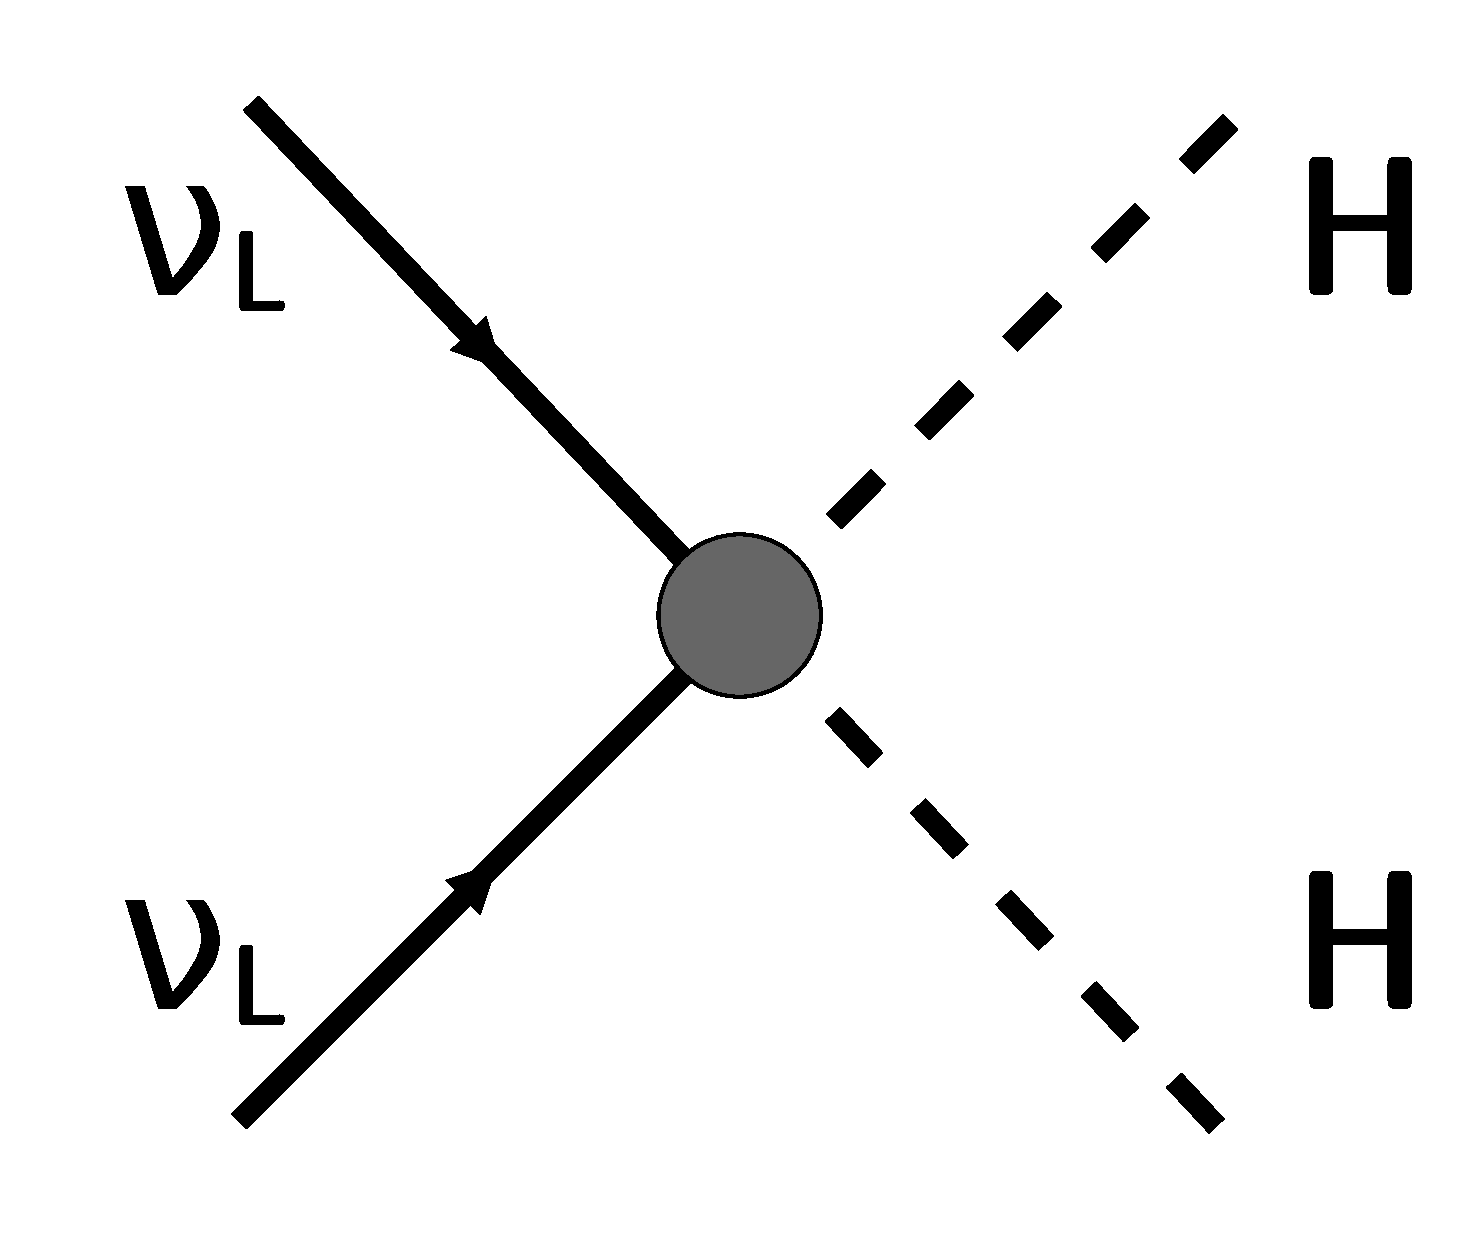
\includegraphics[width=0.3\textwidth]{neutrinophysics/fig_neutrinophysics/Weinberg_diagram.pdf}
  \caption{Weinberg operator diagram.
    The grey circle pictures a new physics interaction.
    \label{fig:weinberg_diagram}}
\end{figure}


\subsubsection{Neutrino mass term}

In the two previous sub-sections the Dirac and Majorana nature of neutrinos were reviewed.
Assuming a right-handed chiral field exists, it is possible to combine the Dirac and Majorana descriptions.
A Dirac-Majorana mass term is derived for one generation of neutrinos, for the minimal model where an additional right-handed neutrino is added to the particle content.


\subsubsection*{Dirac-Majorana mass term}

After Eq.~\eqref{eq:dirac_mass_term}, a Dirac mass term for neutrinos in the Lagrangian can be defined as
\begin{equation}
  \mathcal{L}_D=-m_D\overline{\nu}_L\nu_R+h.c.\,,
  \label{eq:lag_dirac}
\end{equation}
with $m_D=\frac{v}{\sqrt{2}}y^{\,\nu}$ in the case of one generation of neutrinos, where $y^{\nu}$ embeds the Yukawa coupling.
In addition, one can define a Majorana mass term for the right-handed neutrino field as
\begin{equation}
  \mathcal{L}_R=\frac{1}{2}m_R\overline{\nu}_{R}^{\,c}\nu_{R}+h.c.\,,
\end{equation}
with $m_R$ defined in the same manner as in Eq.~\eqref{eq:mass_maj}.
Thus, in general, it is possible to have a Dirac-Majorana mass term in the Lagrangian:
\begin{equation}
\mathcal{L}_{D+M}=\mathcal{L}_D+\mathcal{L}_R=-m_{D}\overline{\nu}_L\nu_R+\frac{1}{2}m_R\overline{\nu}_{R}^{\,c}\nu_{R}+h.c.\,.
\end{equation}
This term can be re-written as
\begin{equation}
  \mathcal{L}_{D+M}=\frac{1}{2}n_L^TC^{\dagger}\mathbb{M}n_L+h.c.\,.
\end{equation}
with $n_L=(\nu_L \nu_R^{c})^{T}$, and the non-diagonal matrix

\begin{equation}
\mathbb{M}=
\begin{pmatrix}
  0 & m_D \\
  m_D & m_{R}
\end{pmatrix}
\,.
\end{equation}
For one generation of neutrinos, $\mathbb{M}$ is a $(2\times 2)$ matrix.
In the more general case of three generations, $m_D$ and $m_R$ are $(3 \times 3)$ diagonal matrices.
The matrix $\mathbb{M}$ has to be diagonalised in order to have masses for $\nu_R$ and $\nu_L$.
$\mathbb{M}$ is diagonalised by $U^T\mathbb{M}U$ with $U$ the mixing matrix from interaction to mass basis
\begin{equation}
  U =
\begin{pmatrix}
  \cos{\theta} & \sin{\theta} \\
  -\sin{\theta} & \cos{\theta}
\end{pmatrix}
\begin{pmatrix}
  \eta_{1} & 0 \\
  0 & \eta_{2}
\end{pmatrix}
\end{equation}
with $\eta_{1}$ and $\eta_{2}$ two phases called Majorana phases, ensuring that masses, eigenvalues of $\mathbb{M}$, are positive.
Thus, after diagonalisation, we have the two masses
\begin{equation}
m_{1,2}=\frac{1}{2}\left(m_R\mp\sqrt{m_R^{2}+4m_{D}^{2}}\right)\eta^{2}_{1,2}\,,
\end{equation}
with $\eta_{1}=i$ and $\eta_{2}=1$.
Here we note the role of Majorana phases: $\eta_{1}$ guarantees the positiveness of the $m_{1}$ solution.
Other models, including a Majorana mass term $m_L$ for the $\nu_L$ field exist, and allow to describe pure Dirac or pure Majorana conditions.


\subsubsection*{See-saw mechanisms}

The Standard Model forbids a mass term for the $\nu_L$ field but predicts nothing for the $\nu_R$ field.
Considering the case were $m_D \ll m_R$ (and $m_L=0$) allows to explain how neutrinos acquire their small neutrino masses, through the see-saw mechanism.
Indeed, the two mass eigenstates can be re-written as
\begin{equation}
  m_1\simeq \frac{m_D^2}{m_R} \qquad \text{and} \qquad m_2\simeq m_R\,.
\end{equation}
If large value is considered for $m_R$ and a small one for $m_D$, the light neutrino has a mass $m_1$ corresponding to the observed active one, while the heavy neutrino has a mass $m_2$ and corresponds to the sterile singlet.
This realisation of the see-saw mechanism is the best known, but others exist.

To introduce a Weinberg operator, leading to a Majorana mass term in the Lagrangian, one can consider the most general form $[L H L H]$, composed of Higgs fields $H$ and lepton fields $L$, and try to combine it in order to have gauge invariant operators.
\begin{itemize}
\item It is possible to combine lepton and Higgs fields to have an $SU(2)$ fermion singlet.
  The corresponding Feynman diagram is represented in Fig.~\ref{subfig:diagram_seesawI}.
  This realisation of the see-saw mechanism was already presented above, where one RH neutrino field gives rise to a mass for one LH neutrino field.
  In that case, the addition of three RH fields to the model would be sufficient to give masses to the three active neutrinos.
\item We can also consider a combination giving a heavy scalar triplet ${\xi = (\xi^{++},\xi^{+},\xi^{0})}$.
  The corresponding Feynman diagram is presented in Fig.~\ref{subfig:diagram_seesawII}.
  This is a mechanism which does not require right-handed neutrinos.
\item The last way to combine lepton and Higgs fields in order to have a gauge invariant Lagrangian consists in introducing a fermionic triplet ${\Sigma = (\Sigma^{+},\Sigma^{0},\Sigma^{-})}$, not to be confused with the baryon of the same name.
  The Feynman diagram is pictured in Fig.~\ref{subfig:diagram_seesawIII}.
\end{itemize}
These three possibilities are in fact the only possible realisations to obtain the effective Weinberg operator, using only renormalisable interactions.
They correspond to the so-called type I~\cite{Minkowski_1977}, II~\cite{Ernest_1998} and III~\cite{Marshak_1980} seesaw mechanisms, respectively.

\begin{figure}[h]
  \centering
  \begin{subfigure}[t]{0.32\textwidth}
    \centering
    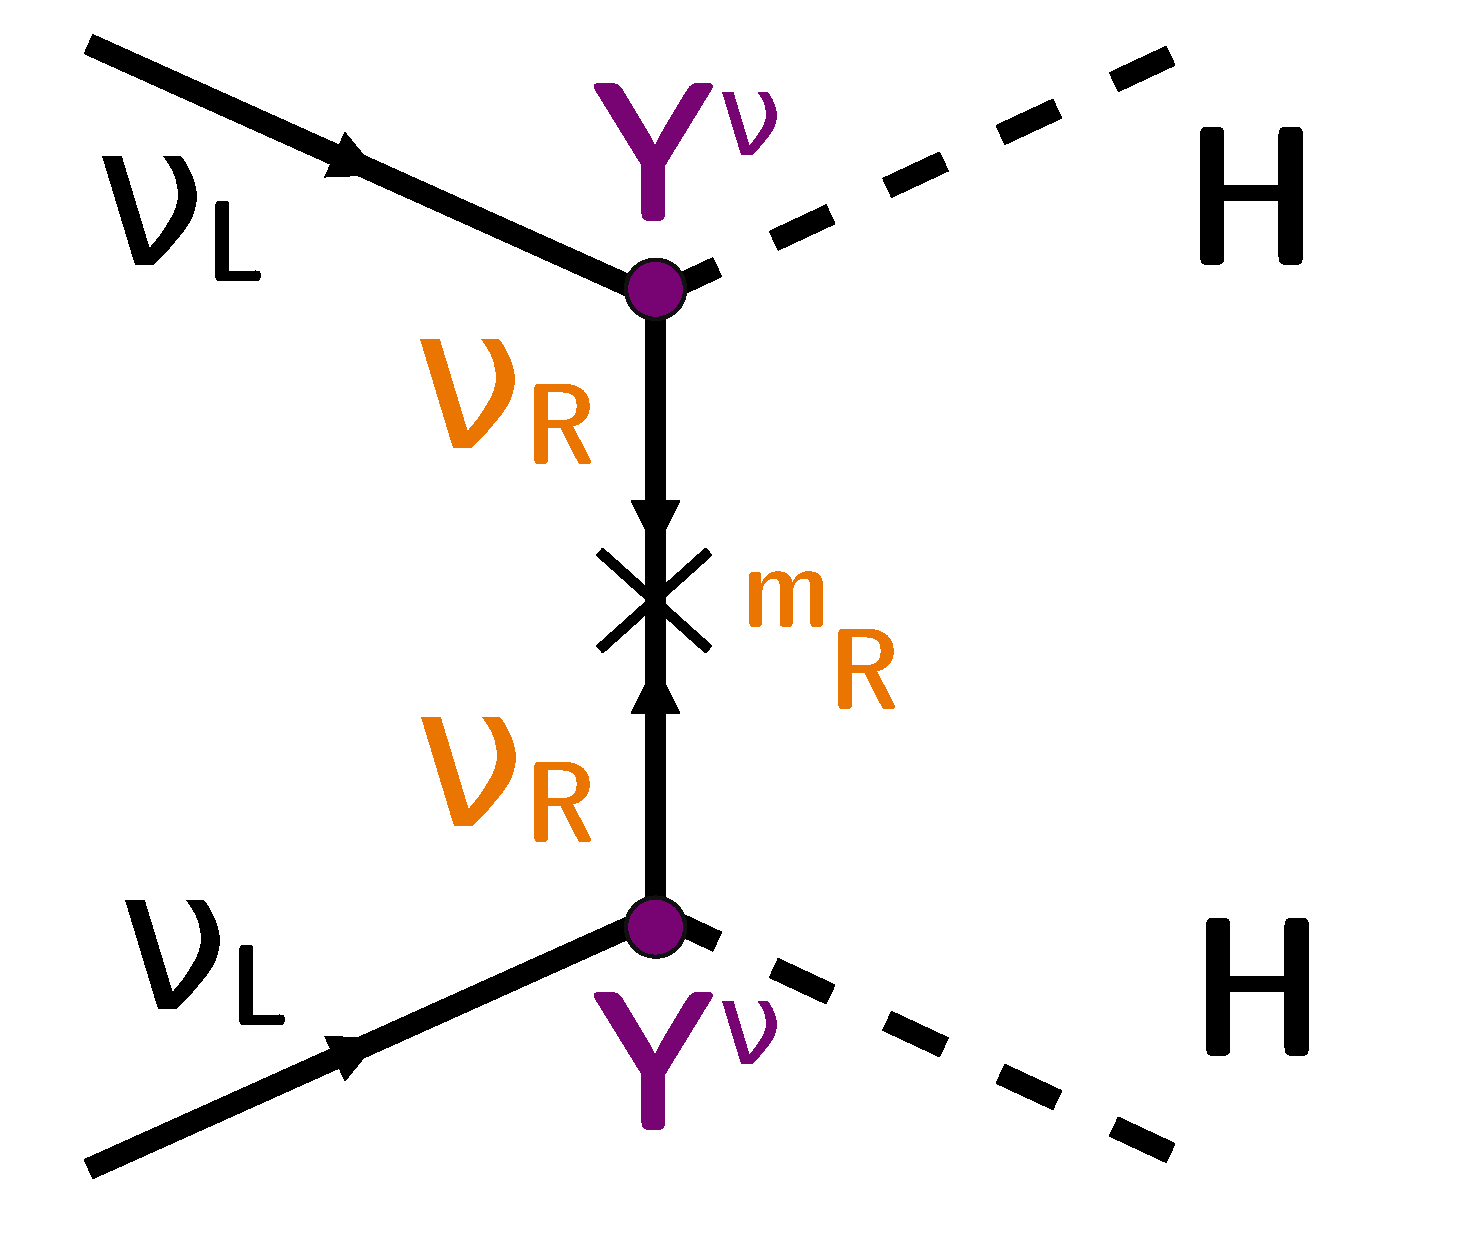
\includegraphics[height=0.7\textwidth]{neutrinophysics/fig_neutrinophysics/seesaw_I.pdf}
    \captionsetup{justification=justified}
    \caption{See-saw type I.
      \label{subfig:diagram_seesawI}}
  \end{subfigure}
  \hfill
  \begin{subfigure}[t]{0.32\textwidth}
    \centering
    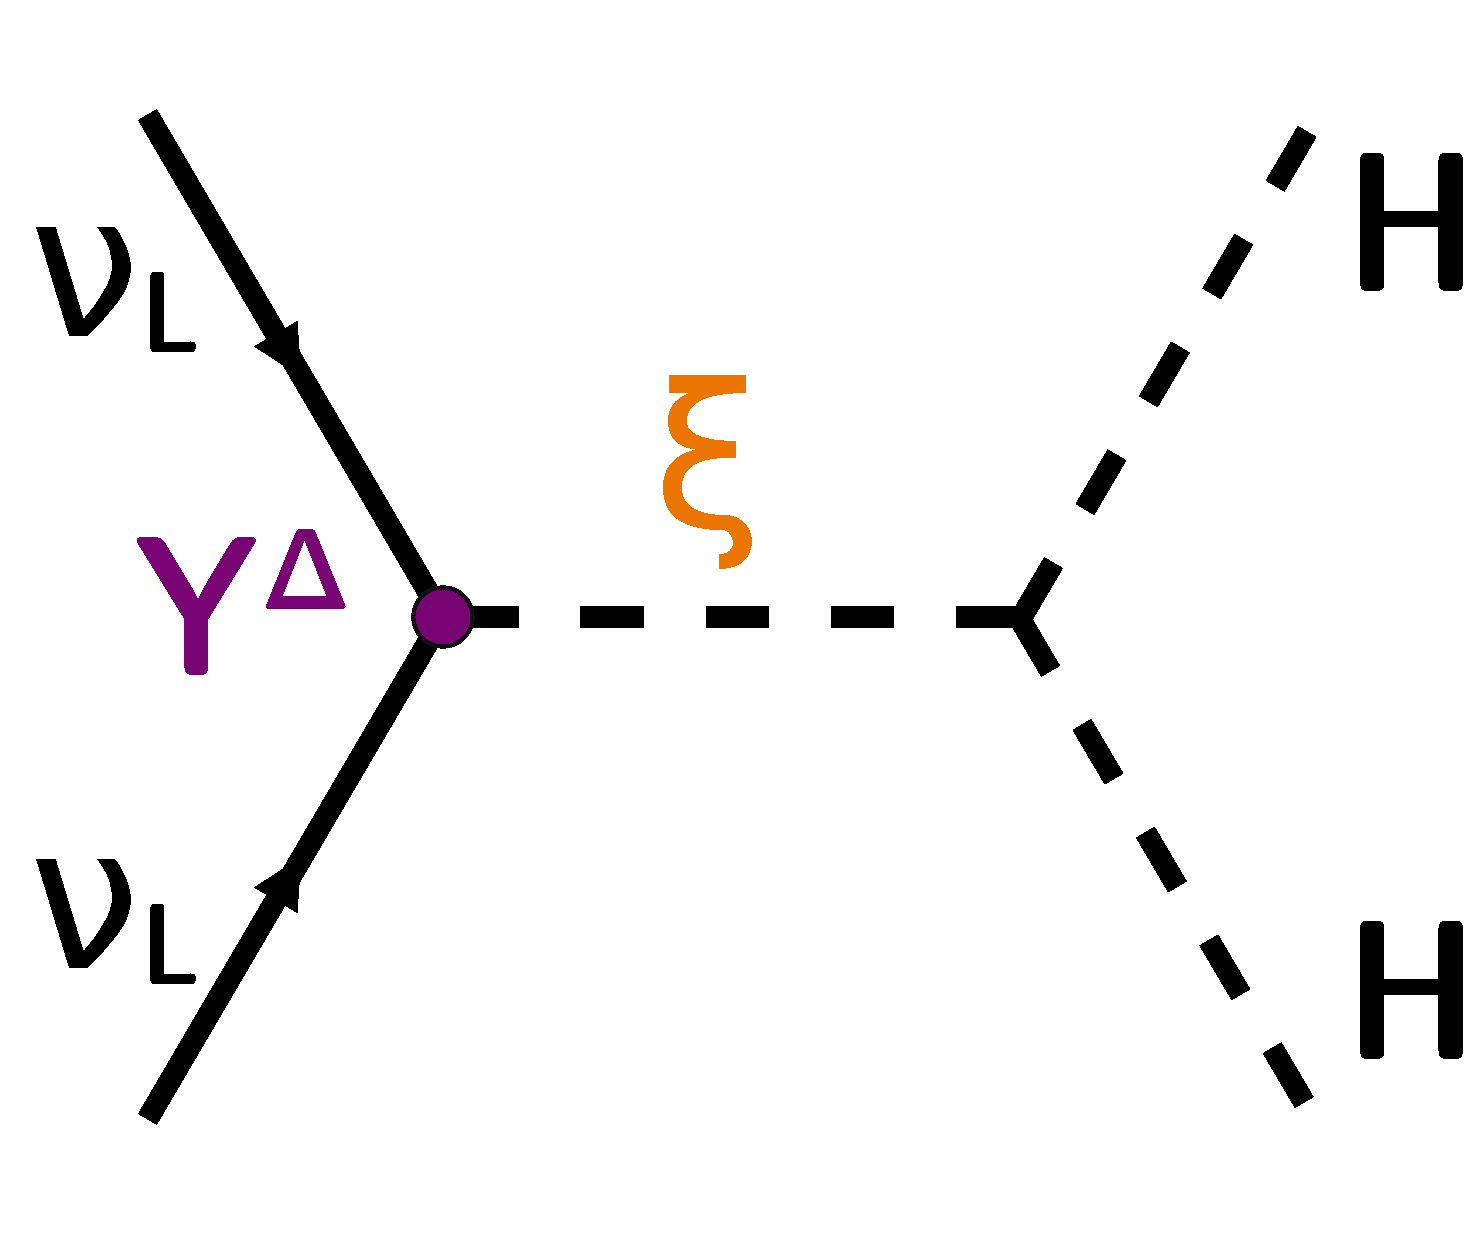
\includegraphics[height=0.7\textwidth]{neutrinophysics/fig_neutrinophysics/seesaw_II.pdf}
    \captionsetup{justification=justified}
    \caption{See-saw type II.
      \label{subfig:diagram_seesawII}}
  \end{subfigure}
  \hfill
  \begin{subfigure}[t]{0.32\textwidth}
    \centering
    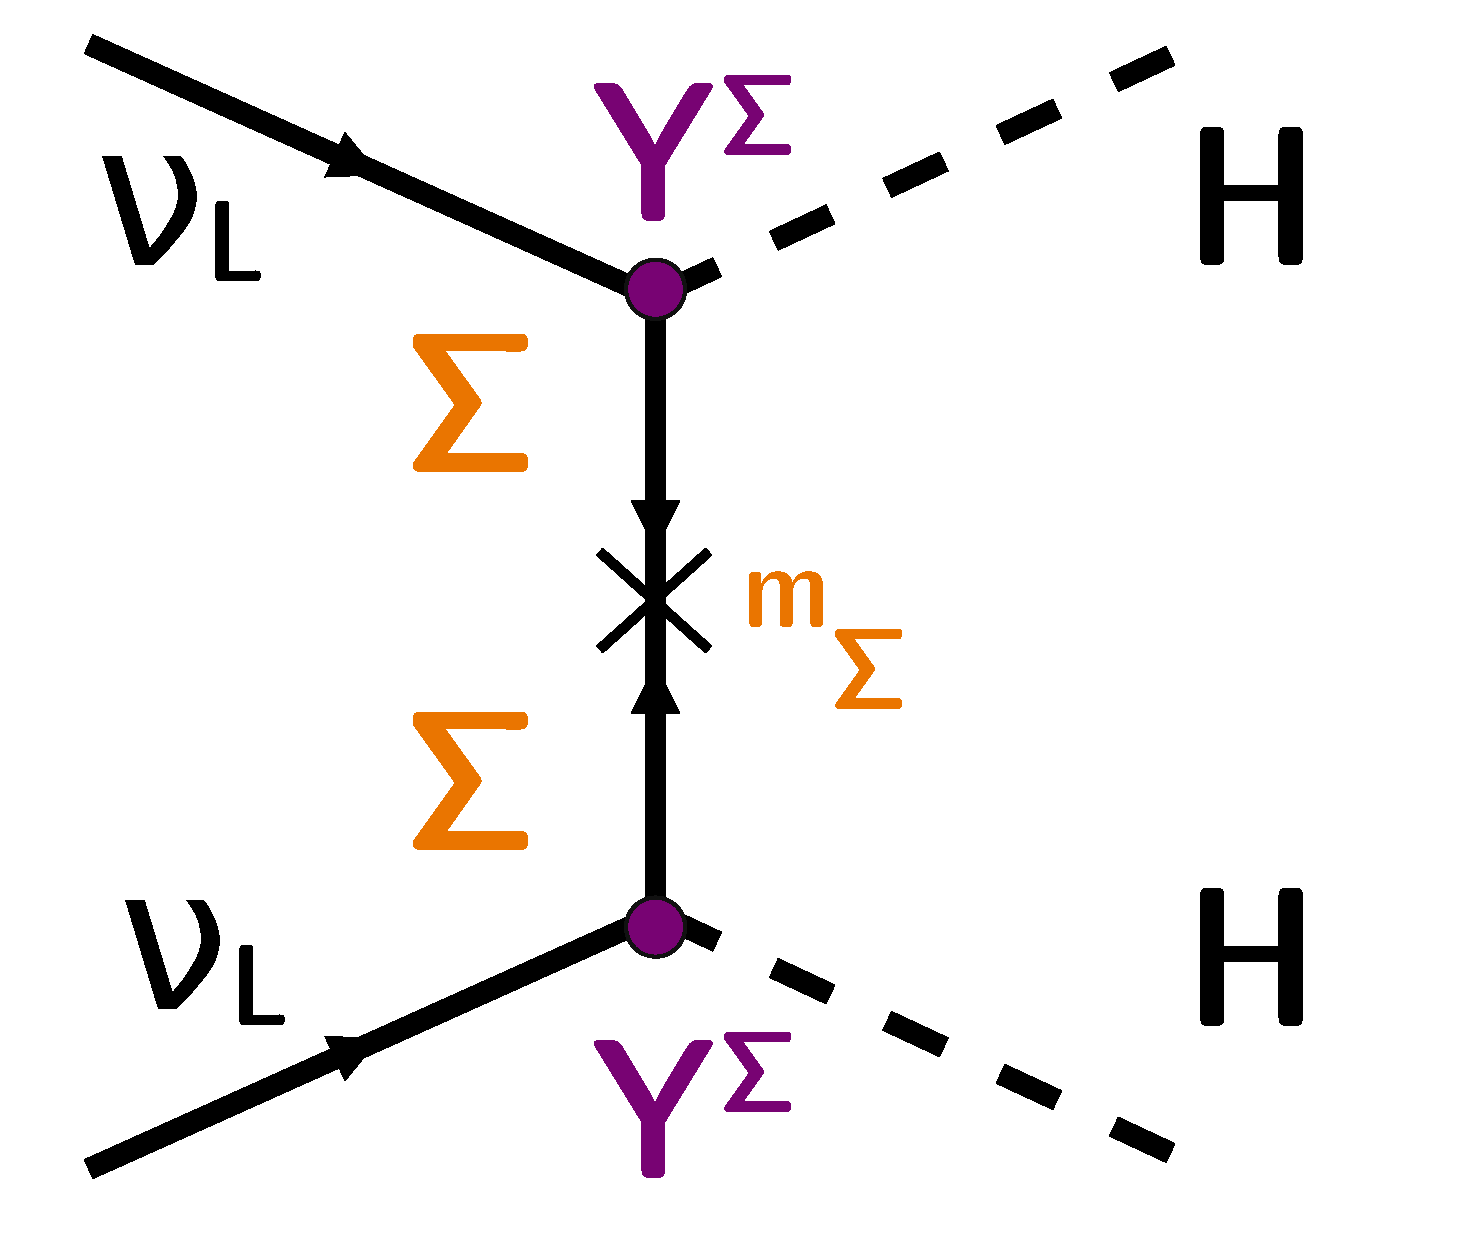
\includegraphics[height=0.7\textwidth]{neutrinophysics/fig_neutrinophysics/seesaw_III.pdf}
    \captionsetup{justification=justified}
    \caption{See-saw type III.
      \label{subfig:diagram_seesawIII}}
  \end{subfigure}
  \caption{
    \label{fig:diagram_seesaws}
  }
\end{figure}



\subsection{Double beta decays}
\label{subsec:double_beta_decays}


Even though it is not protected by a symmetry, the total lepton number is conserved in the SM.
If the neutrino is found to be a Majorana particle it could open leads for the explanation of lepton number violation, the small masses of the neutrinos through the see-Saw mechanism and the matter/antimatter asymmetry in the Universe through Leptogenesis.
Should neutrinos be Majorana particles, their mass term leads to lepton number violation (LNV), with $\Delta L = 2$.
The best known process able to probe LNV is neutrinoless double beta decay~\cite{art:Drewes_2013}.



\subsubsection*{Standard double beta decay}

Let us first introduce the double beta decay proposed by Goeppert-Mayer in $1935$~\cite{art:goeppert_1935} as
\begin{equation}
(A,Z)\rightarrow (A,Z+2)+2e^{-}+2\overline{\nu}_{e}\,,
\end{equation}
describing two simultaneous $\beta$ decays of two nucleons of the same nucleus.
This decay is physically possible for nuclei with an even-even number of nucleons, for whose a simple beta decay would not be favourable: the energy of the daughter nucleus would be higher than the parent one.
In some cases (as the $^{48}$Ca nucleus) the simple $\beta$ decay is suppressed because of transition spin considerations.
This transition is strongly suppressed which makes it the rarest known nuclear decay (see Fig.~\ref{fig:2nu_even_odd}).
It is allowed by the Standard Model for $35$ isotopes, and despite its rarity, has already been observed for numerous of them like \Mo, \Se, $^{136}$Xe and $^{76}$Ge, with typical half-lives ranging from $10^{18}$ to $10^{24}$~years.
The Feynman diagram illustrating this process is given in Fig.~\ref{fig:2nu_diagram}.

\begin{figure}[h]
  \centering
  \begin{subfigure}[t]{0.48\textwidth}
    \centering
    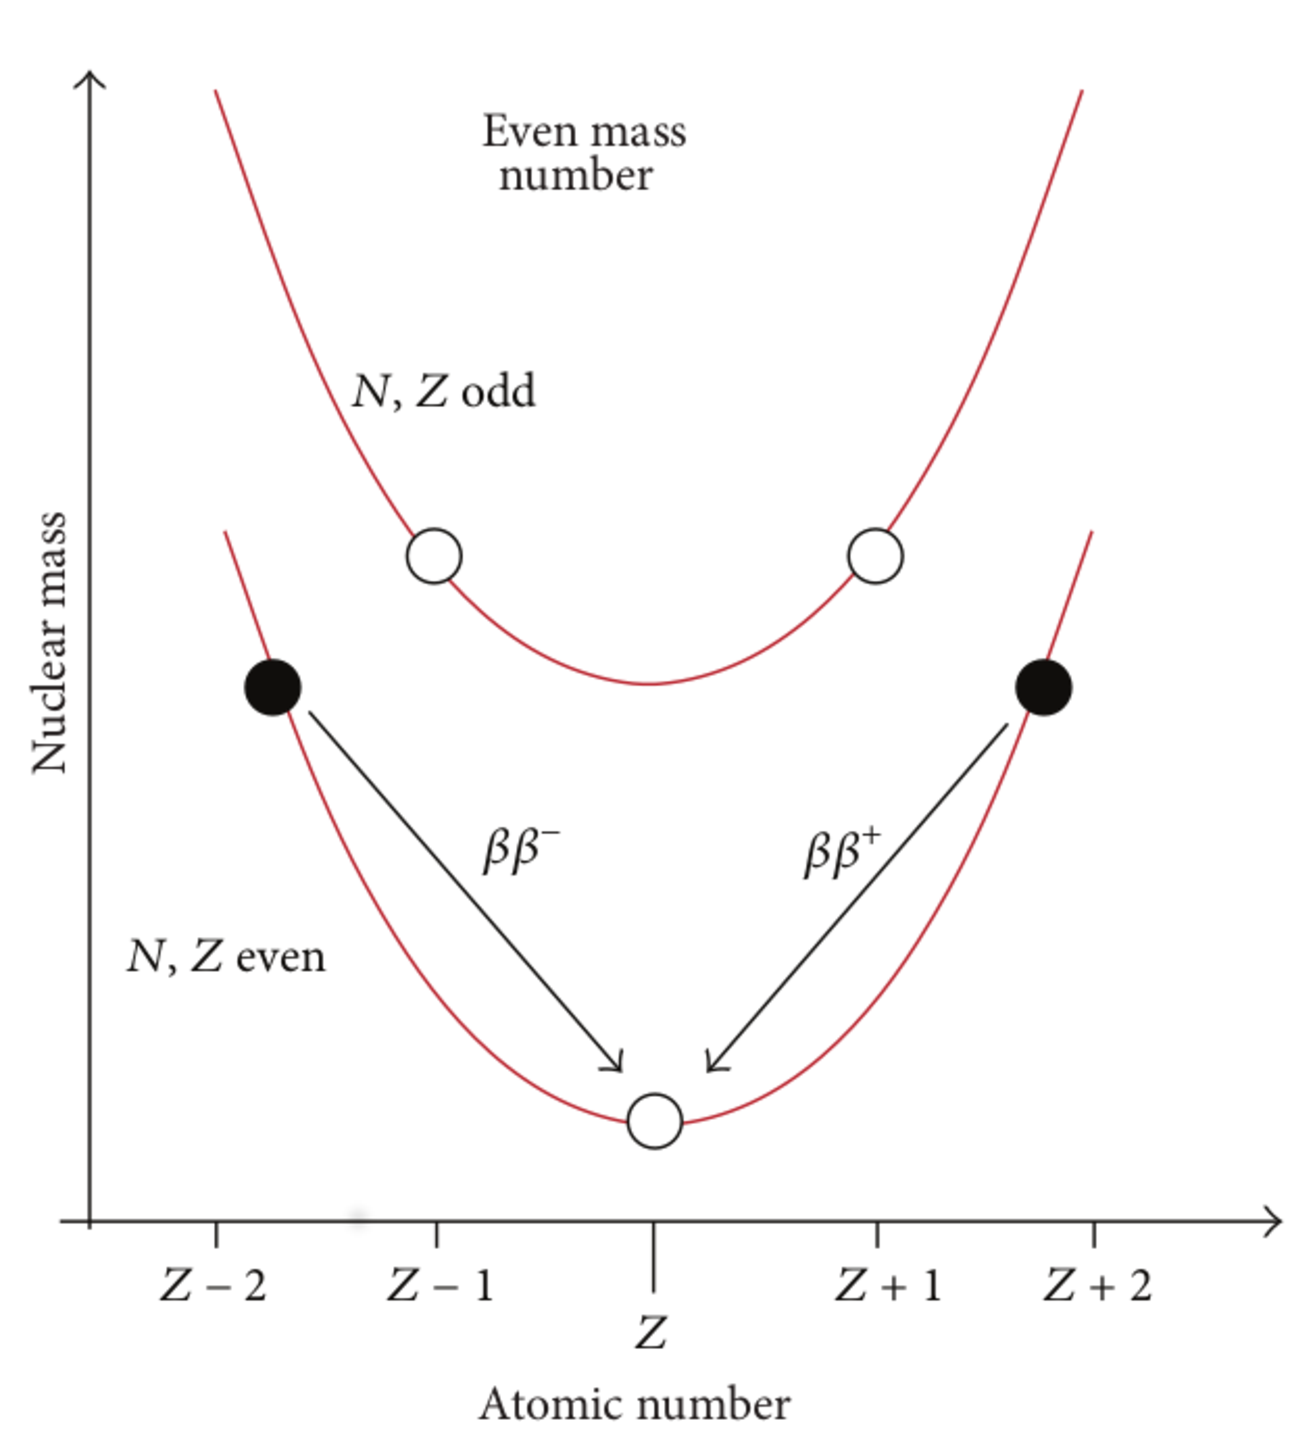
\includegraphics[width=1\textwidth]{neutrinophysics/fig_neutrinophysics/2nu_even.pdf}
    \captionsetup{justification=justified}
    \caption{
      \label{subfig:}}
  \end{subfigure}
  \hfill
  \begin{subfigure}[t]{0.48\textwidth}
    \centering
    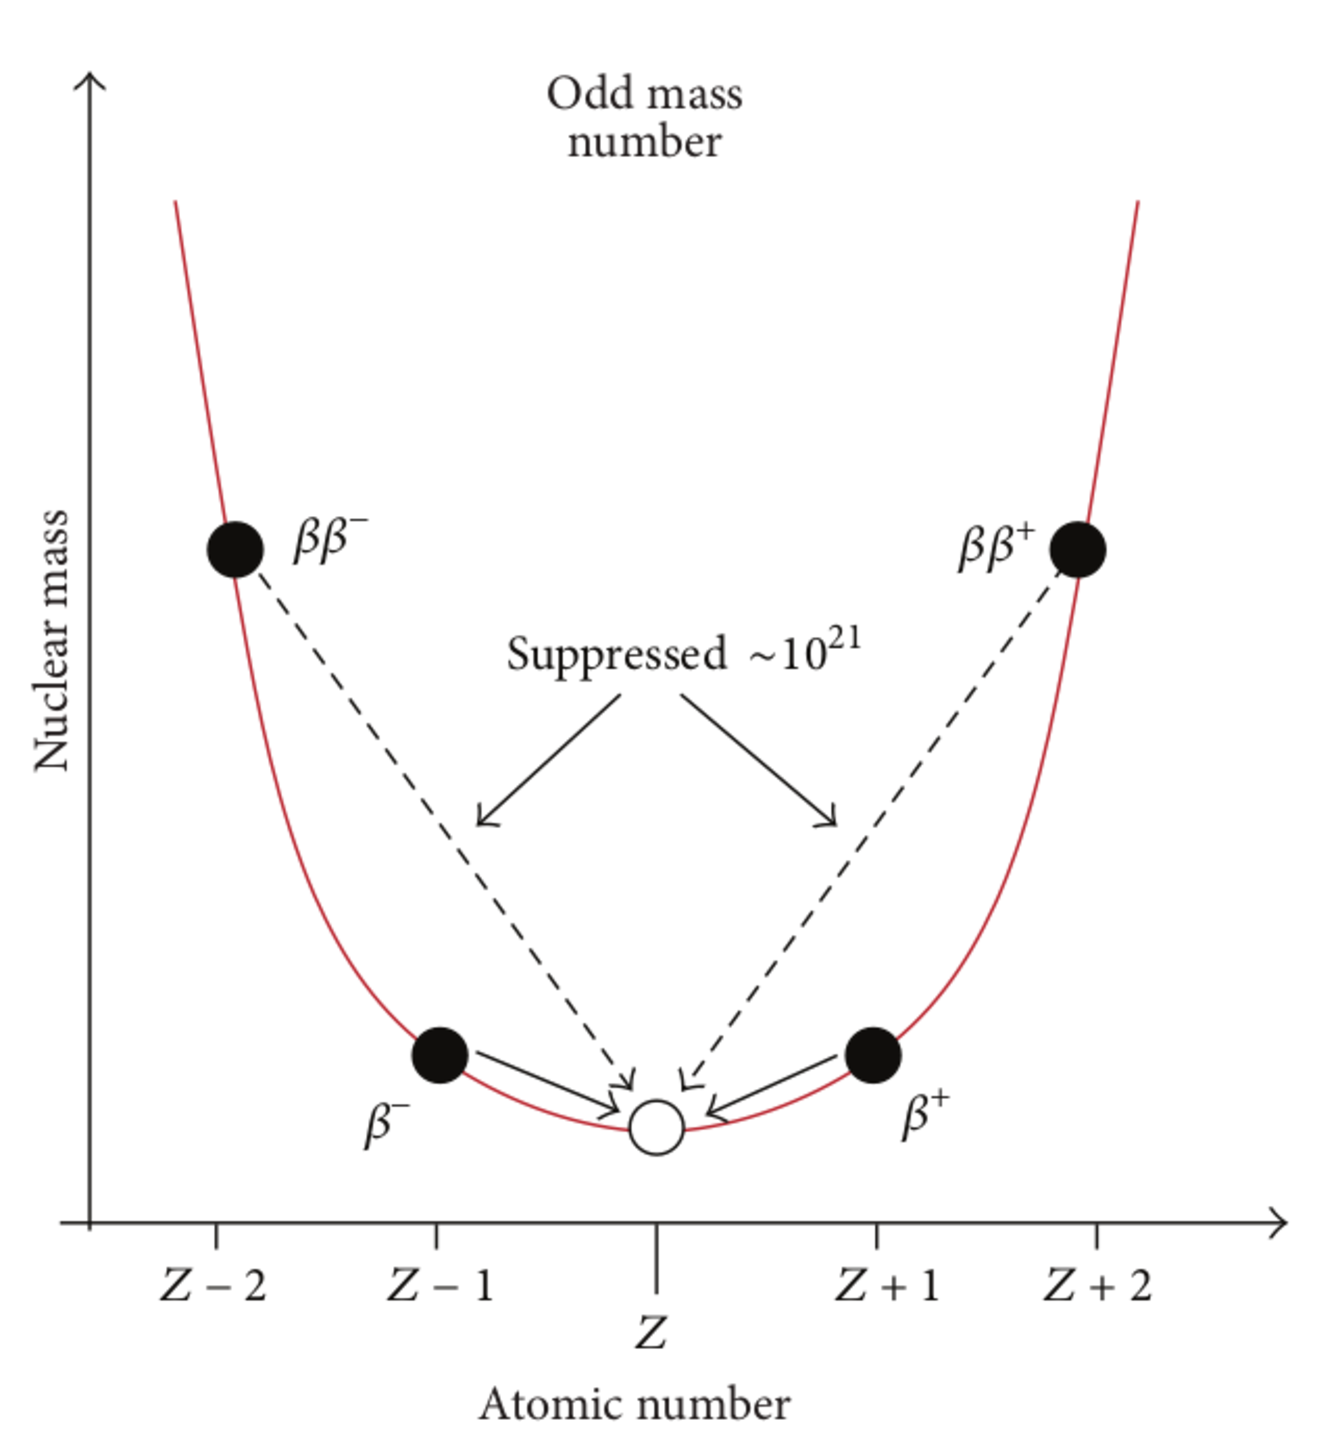
\includegraphics[width=1\textwidth]{neutrinophysics/fig_neutrinophysics/2nu_odd.pdf}
    \captionsetup{justification=justified}
    \caption{
      \label{subfig:}}
  \end{subfigure}
  \caption{Nuclear mass as a function of the atomic number $Z$ in the case of an isotope with $A$ even (a) and $A$ odd (b).
    Adapted from~\cite{art:delloro_2015}.
    \label{fig:2nu_even_odd}
  }
\end{figure}

\begin{figure}[h!]
  \centering
    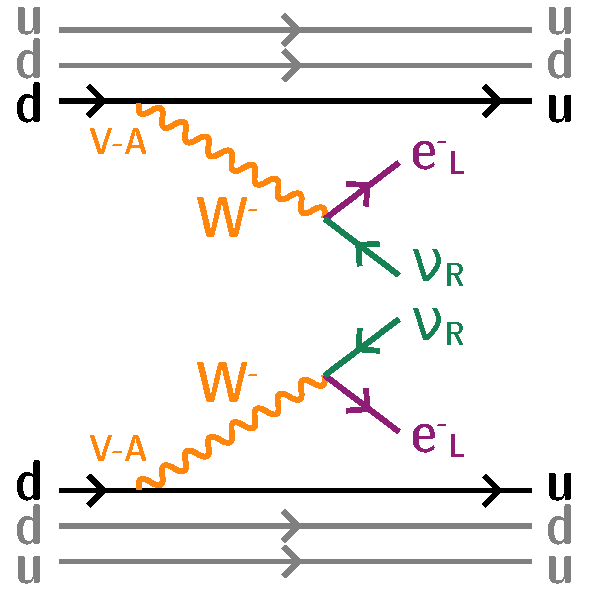
\includegraphics[height=0.4\textwidth]{neutrinophysics/fig_neutrinophysics/2nubb_diagram.pdf}
  \caption{Standard double beta decay.
    \label{fig:2nu_diagram}}
\end{figure}


\subsubsection*{Neutrinoless double beta decay}

In $1939$, Furry~\cite{art:furry_1939} proposed the double beta decay without neutrino production as
\begin{equation}
(A,Z)\rightarrow (A,Z+2)+2e^{-}\,,
\end{equation}
in which two neutrons simultaneously decay into protons.

The existence of such a decay would have deep implications for various physics research.
Firstly, as neutrinos are not emitted, this process implies the violation of the total lepton number by $2$ units, thus making it forbidden in the SM.
However, the lepton number conservation results from an accidental symmetry breaking of the SM, and thus its violation would not necessarily imply Physics beyond the Standard Model.
But more than the LNV, the $\zeronu$ would violate also the baryon - lepton number (B-L) which, on the contrary, is a fundamental symmetry of the SM.
Hence such observation would have major contribution for theories trying to explain the matter/antimatter asymmetry of the Universe.
Moreover, the $\zeronu$ process is allowed only if neutrinos are massive Majorana particles.
Therefore, the observation of this decay would point to the existence of a process that violates a fundamental symmetry of the Standard Model of Particle Physics, and would allow to establish the nature of neutrinos.

At the moment, no experiment has observed $\zeronu$ processes, but various experiments, of which a non-exhaustive list is given in Sec.~\ref{sec:0nu_exp}, have lead to precise limits on $\zeronu$ half-life of $10^{25}-10^{26}$~years.
The future generation of $\zeronu$ experiment is currently under construction.

The absence of neutrino emission, if detected experimentally, would prove the Majorana nature of the neutrino.
The underlying mechanism through which the neutrinoless double beta decay would occur is not known, and several theories have been developed.
\begin{itemize}
\item Higher dimensional operators: the dimension-$5$ Weinberg operator presented above is the lowest dimension operator that can be built for the mass of Majorana.
  In addition, it is possible to consider higher dimension operator (dimension $6$ and $9$ for instance), that are effective and non-renormalisable, respecting the gauge symmetry ${SU(3)_C\times SU(2)_L\times U(1)_Y}$.
\item Heavy neutrino exchange considers the case where a heavy RH neutrino is exchanged during the $\zeronu$ decay.
  This was historically the first case to be considered, including a dimension-$9$ operator, with constraints on the heavy neutrino mass with the mixing between left-handed neutrinos and the heavy neutrino.
\item Right-handed currents include new RH gauge bosons $W_R$ of a new $SU(2)_R$ gauge group.
  The corresponding operator would be of dimension-$9$ and highly suppressed, by $4$ powers of the masses of the new gauge bosons.
\end{itemize}
In Fig.~\ref{fig:0nu_diagram} is given the Feynman diagram of the neutrinoless double $\beta$ decay for the light Majorana neutrino exchange realisation.

\begin{figure}[h!]
  \centering
    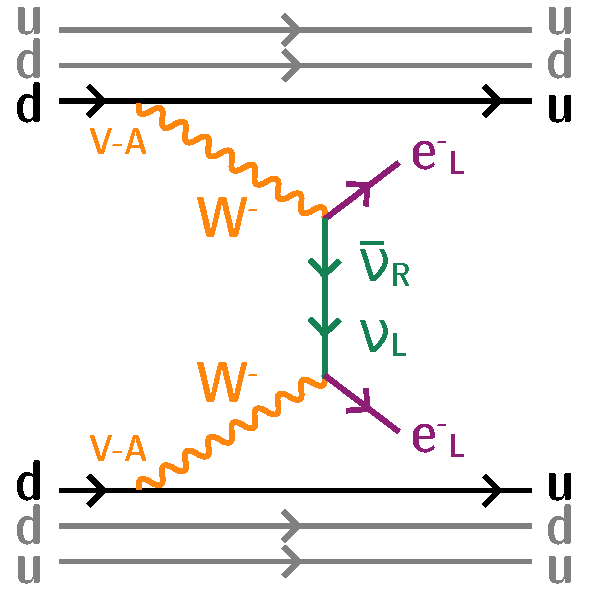
\includegraphics[height=0.4\textwidth]{neutrinophysics/fig_neutrinophysics/0nubb_diagram.pdf}
  \caption{Neutrinoless double beta decay through light Majorana neutrino exchange.
    \label{fig:0nu_diagram}}
\end{figure}

\subsubsection*{Experimental search for $\zeronu$}

One of the experimental observable of the double $\beta$ decays is the total energy spectrum of the $2$ emitted electrons, given in Fig.~\ref{fig:bb_energy}.
The $\twonu$ decay emits $4$ leptons, the two electrons having an energy continuum between $0$ and $\Qbb$, the total availbale energy of the reaction.
In the case of the $\zeronu$ decay, the two electrons would bring the total energy of the reaction, thus the expected signature would be an energy peak at $\Qbb$.

If existing, the $\zeronu$ decay would be an extremely rare process.
The decay rate of the light Majorana exchange is given by:
\begin{equation}
  (T_{1/2}^{0\nu})^{-1} = g_{A}^{4}G^{0\nu}|M^{0\nu}|^{2}\left\lvert\dfrac{m_{\beta\beta}}{m_{e}}\right\rvert^{2}\,.
\end{equation}
where $G^{0\nu}$ is the phase space factor embedding the influence of the Coulomb field of the daughter nucleus on the emitted electrons/positrons.
$M^{0\nu}$ is called the nuclear matrix element embedding the nuclear structure effects of the decaying nucleus.
$m_{\beta\beta}$ is the effective neutrino mass defined as
\begin{equation}
  \langle \mbb \rangle = \left\vert \sum_{i=1...3}m_{i}U^{2}_{ei} \right\vert \,,
\end{equation}
is summed over the three mass eigenstates.
This effective mass depends on the $U_{PMNS}$ matrix elements given in~\ref{eq:upmns_detail}, and thus is a function of the CP violating phases and of the mass ordering.

\begin{figure}[h!]
  \centering
    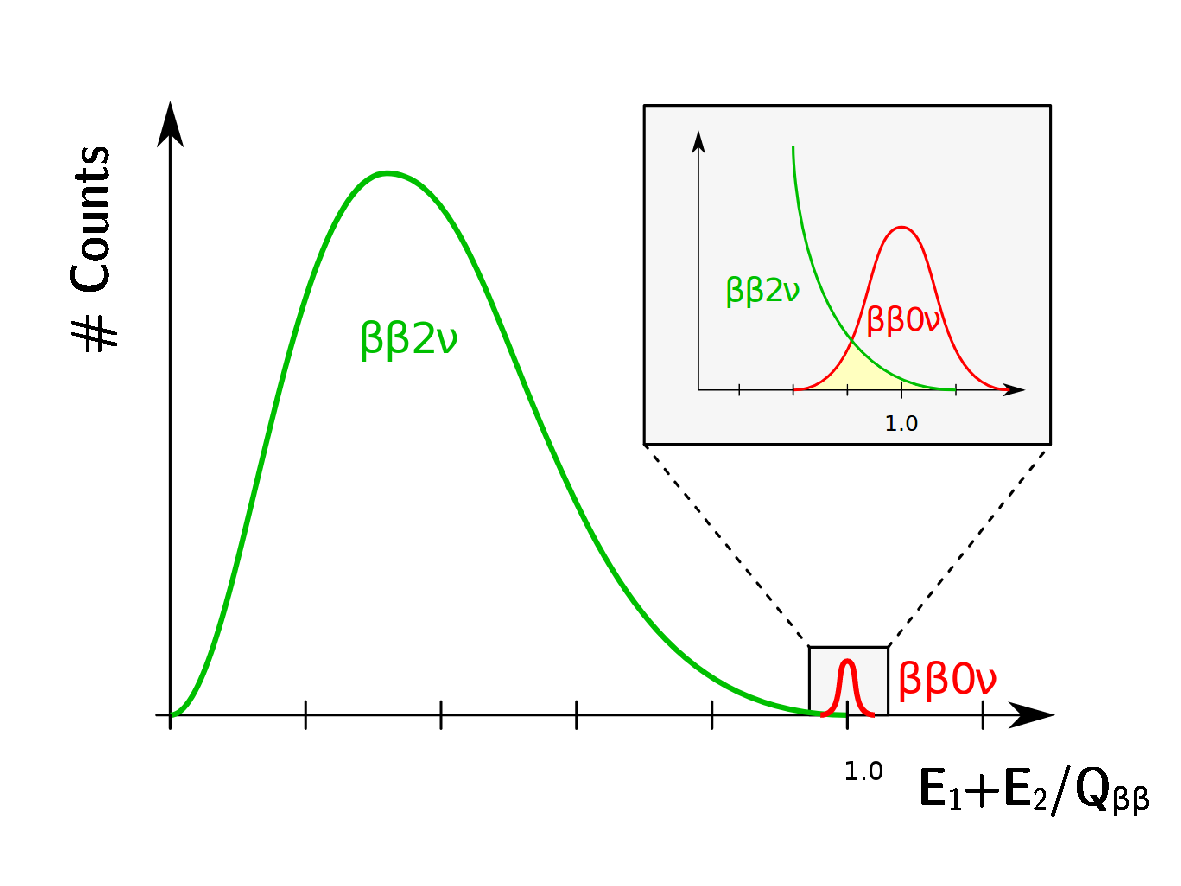
\includegraphics[height=0.6\textwidth]{neutrinophysics/fig_neutrinophysics/reconstructed_energy.pdf}
  \caption{
    \label{fig:bb_energy}}
\end{figure}



\section{$\zeronu$ experimental status}
\label{sec:0nu_exp}

\subsection{Experimental design criteria}

As no neutrinos are emitted in a $\zeronu$ decay, the minimal observable in direct searches for $\zeronu$ decay is the total energy of the two emitted electrons.
Depending on experiment designs and purposes (detailed in Sec.~\ref{sec:zeronuexp}), individual electron energies and tracks also represent interesting observables.
The signature of a $\zeronu$ signal is an excess of events, compared to the expected background noise, in the total energy spectrum, near the $\Qbb$ released energy.
How large is this peak depends on the energy resolution of the detector.
Research for this signal involves optimising a \emph{region of interest} (ROI), also depending on the energy resolution.
The total number of events $N^{0\nu}$ occurring in the ROI and in the measurement time $t$, for a detector with an detection efficiency $\epsilon$, using a source isotope of $W$ atomic molar mass and $a$ isotopic abundance, is defined as
\begin{equation}
  N^{0\nu}=\ln(2)\frac{\mathcal{N}_{A}}{W}\left(\frac{a\epsilon M t}{\Tbeta}\right)\,\text{,}
  \label{eq:Nevents}
\end{equation}
where $\mathcal{N}_{A}$ is the Avogadro number.
If no excess of events is observed, the limit set on the $\zeronu$ decay half-life is
\begin{equation}
  T_{1/2}^{0\nu\text{,lim}}=\ln(2)\frac{\mathcal{N}_{A}}{W}\left(\frac{a\epsilon M t}{N_{\text{exc}}}\right)\,\text{,}
  \label{eq:Tlim}
\end{equation}
$N_{\text{exc}}$ being the number of $\zeronu$ events excluded at a given confidence level in the ROI.
Then, this sensitivity to the $\zeronu$ decay would depend on the number of total counts in the ROI, some of them possibly being background events:
\begin{equation}
  T_{1/2}^{0\nu\text{,lim}} \propto \left\{
  \begin{array}{ll}
    a M \epsilon t & \text{if no background is expected,} \\
    a \epsilon \sqrt{\frac{M t}{B \Delta E}} & \text{with background.}
  \end{array}
  \right.
  \label{eq:sensitivity_background}
\end{equation}
Here $B$ is the background rate usually expressed in $\Bckunit$ (when normalised to the width of the ROI, the source mass, and the observation time) and $\Delta E$ is the energy resolution.
The advantage of a background free experiment clearly comes out: the $\zeronu$ half life would increase linearly with the time of exposure $t$ (as opposed to $\sqrt t$ for an experiment with a large number of background events).
Then, it is clear that the control and the discrimination of background is of high priority for such $\zeronu$ direct search experiments.
We will discuss in Chap.~\ref{ch:detector} some important point to reduce the backgrounds for the $\zeronu$ decay detection.
Next to that, the previous expression fixes the choices that experimenters can make in designing a detector.
An ideal isotope would have a high natural abundance and would be deployed with the highest mass possible in a detector with a high detection efficiency, a good energy resolution (small $\Delta E$) under low-background conditions (small $B$).
Of all the $35$ isotopes capable of disintegrating through $\twonu$, none meets all the previous conditions.
Experimenters will then have to find compromises, which are at the origin of the different detection strategies.
Detector can ether use an active or passive source.
In the first case, the source is also the detection medium (detector technologies detailed in Sec.~\ref{subsec:semiconductors},~\ref{subsec:bolometers} and~\ref{subsec:scintillators}).
In the second case, the source is decoupled from the detection part of the experiment (see Sec.~\ref{subsec:TPC} and~\ref{subsec:trackocalo}).
In the next section, we provide a review of the current and future experiments that aim to discover the neutrinoless double beta decay.


\subsection{$\zeronu$ direct search experiments}
\label{sec:zeronuexp}
\subsubsection{Semiconductors}
\label{subsec:semiconductors}
Various semiconductor technologies are employed in the detection of $\zeronu$ decay.
The $^{76}$Ge $\beta\beta$ emitter ($\Qbb=2039$ keV) is historically important as it has been adopted since the 1960s in $\zeronu$ decay searches, acting as active source, which enhances the detection efficiency.
$^{76}$Ge-enriched high purity Germanium detectors (HPGe) offer both high energy resolution and extremely high radiopurity (as impurities are removed in the crystal growing process).
These characteristics allow, once external background contribution is minimised, to reach high sensitivity on $\zeronu$ decay, which makes this category of detectors one of the most promising for ton-scale experiments.
Since the last generation (IGEX and Heidelberg-Moscow), HPGe detectors had been improved to reach an ultra low background rate, making way for the current generation of $\zeronu$ detectors -- GERDA, MAJORANA demonstrator and LEGEND.

\paragraph{GERDA} experiment (GERmanium Detector Array) is located at the Laboratori Nazionali del Gran Sasso (LNGS), Italy.
GERDA phase I was running from $2011$ to $2013$ with $17.8$ kg of enriched active source detectors from the HEIDELBERG-MOSCOW and IGEX experiments.
Its first aim was to put to the test the controversial result of HEIDELBERG-MOSCOW experiment given in $2001$, announcing the first evidence for $\zeronu$ signal at a $4.2\sigma$ confidence level.
With an exposure of $21.6$ kg.y, the absence of signal in the GERDA-I experiment refuted the previous result, setting a limit $\Tbeta>2.1\, 10^{25}$ y.
Since $2015$, the GERDA experiment is in the second phase (see Fig.~\ref{fig:GERDA}), with a total of $35.8$ kg enriched detectors, $20$ kg of which is Broad Energy Germanium (BEGe) detectors that have been deployed for GERDA-II, providing a better energy resolution and pulse shape discrimination.
The active source is deployed inside a liquid Argon (LAr) augmented with light sensors, acting as an active external shield as well as a cooling down system.
The total is surrounded by a water tank.
The aim is to reach a $10^{26}$ y sensitivity with $100$ kg.y exposure, and a background rate less than $10^{-3}$ $\Bckunit$.
The underground laboratory of INFN provides $3500$ m water equivalent to reduce the external cosmic background.
In $2019$, a combined analysis for GERDA phases I and II has resulted in a half-life limit of $\Tbeta>9\, 10^{25}$ y ($90$\% C.L., sensitivity assuming no signal is $1.1\, 10^{26}$), corresponding to an effective neutrino mass of $\mbb<0.07\text{-}0.16$ eV ($90$\% C.L.).

\begin{figure}
  \centering
  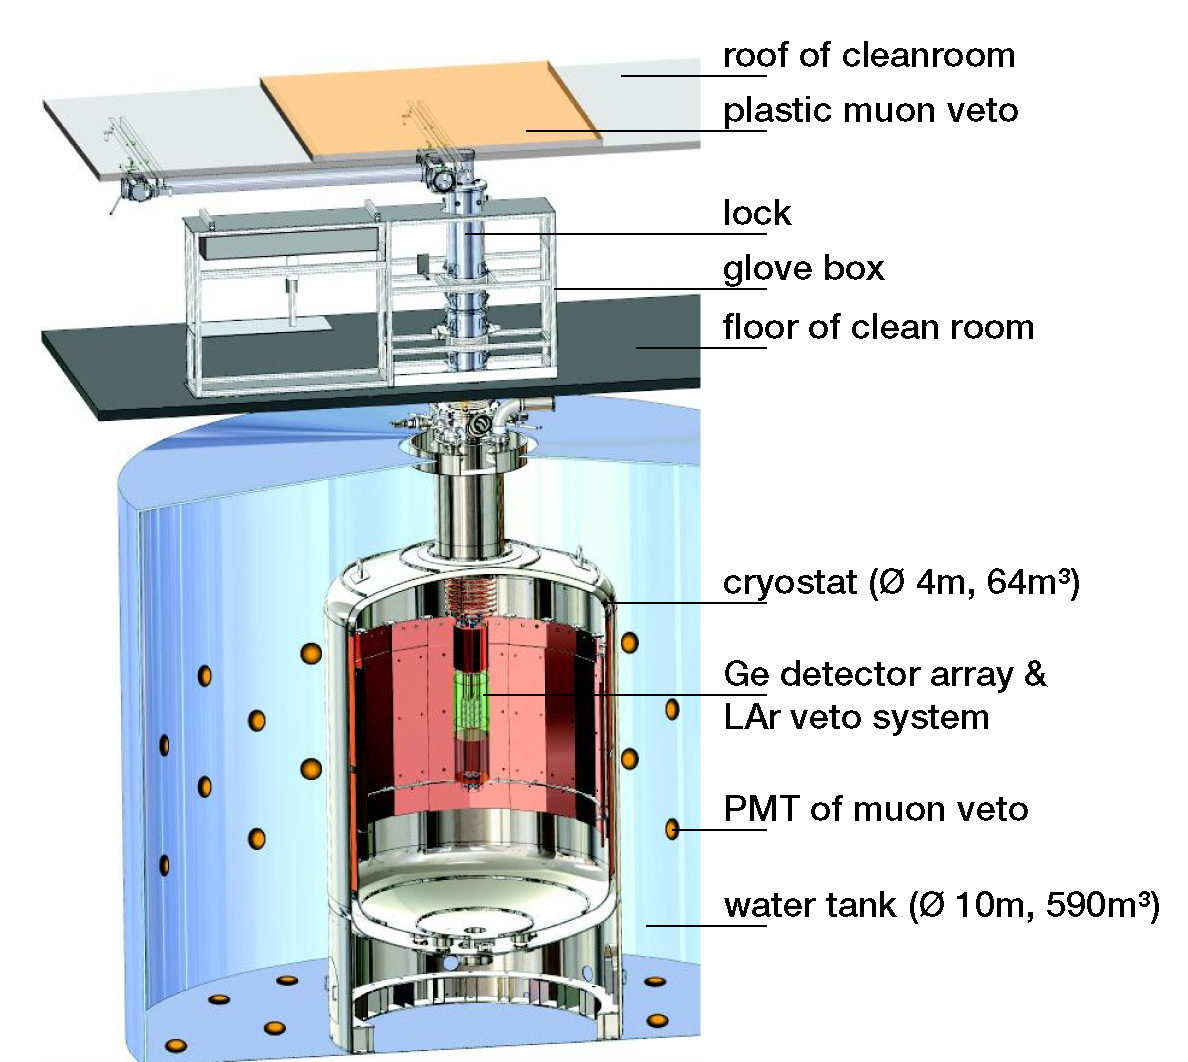
\includegraphics[width=10cm]{neutrinophysics/fig_neutrinophysics/GERDA.png}
  \caption{Scheme of the GERDA experiment.
    \label{fig:GERDA}}
\end{figure}


\paragraph{MAJORANA demonstrator} is an array of enriched germanium detectors that searched for the $\zeronu$ decay of the $^{76}$Ge isotope, using High Purity Germanium (HPGe) detectors.
The Majorana Demonstrator is located at the Sanford Underground Research Facility (SURF) in Lead, USA.
It is composed of $58$ HPGe detectors divided into $2$ cryostats with $7$ strings each.
Each string is an assembly of $3$, $4$ or $5$ detectors.
The total mass of HPGe crystals is $44.1$~kg, $29.7$~kg of which is enriched to $88$\% $^{76}$Ge.
The observed lower limit is $\Tbeta>2.7\times 10^{25}$~years at $90$\% CL~\cite{art:majorana2019}.
A combined limit from the two Ge-based experiments GERDA and MAJORANA would exceed $10^{26}$~years.

\paragraph{LEGEND} for Large Enriched Germanium Experiment for Neutrinoless Double-Beta Decay.
After the encouraging results of the MAJORANA Demonstrator and GERDA, the LEGEND collaboration has been formed to pursue a tonne-scale $^{76}$Ge experiment, with discovery potential at a half-life beyond $10^{28}$~years.
The collaboration aim to use existing material from GERDA, especially the cryostat, and perform additional R\&D to build the detector.

\subsection{Bolometers}
\label{subsec:bolometers}

Bolometers are high energy resolution and high detection efficiency calorimeters operating at low temperatures ($\simeq 10-20$ mK), by measuring the heat increase, quantified by phonons, generated by particles interaction in the crystal.
This technology provides a good energy resolution of few keV.
The crystals are both the source and the detector, which is particularly suitable for $\zeronu$ searches, and provides the possibility to build large-scale experiments.
As the two electrons topology is not available, analyses of the pulse shapes can be perfomed in order to discriminate the signal from the electronics noise and the natural radioactivity events.

\paragraph{CUORE} for Cryogenic Underground Observatory for Rare Events, is an experiment based at Laboratori Nazionali del Gran Sasso in Italy.
The feasibility of the project has been proved by Cuoricino, the pilot experiment taking data from $2003$ to $2008$ with $62$ TeO$2$ cryogenic detectors, for a total of $19.75$~kg.y exposure, achieving a lower limit of $\Tbeta>2.8\times 10^{24}$~years at $90$\% CL.
The next step towards the final experiment CUORE was CUORE-$0$, aiming at improve the background reduction.
The data took place from $2013$ to summer $2015$, showing the $\alpha$ background were reduced by a factor $6$.
The CUORE detector consists of an array of $988$ TeO$2$ crystals arranged in a cylindrical structure of $19$ towers.
The first results of the CUORE experiment had been published in $2018$, where no evidence for $\zeronu$ were found.
Combining their results with the earlier experiments Cuoricino and CUORE-$0$, a lower limit of $\Tbeta>1.5\times 10^{25}$~years at $90$\% CL were achieved.



\paragraph{CUPID} for CUORE Upgrade with Particle IDentification, uses the expertise acquired with CUORE facility, with a background level improved by a factor $100$, as the particle identification is a powerful tool for background rejection.


\paragraph{AMoRE}
\subsection{Time projection chambers}
\label{subsec:TPC}

Time Projection Chambers (TPC) detectors use a medium producing two ways to measure the electron energies: a \emph{scintillation} (ultra-violet light) prompt signal, and a \emph{ionisation} delayed signal.
When a particle crosses the detector, a scintillation light is emitted, the energy of the scintillation peak depending on the medium.
Scintillation photons, travelling at speed of light in the medium, are detected by photo-sensors, giving the \emph{zero-time} of the event.
The crossing particle ionises the medium all along its way, creating electrons drifting to a collection system (an electric field is applied between cathode and anode), allowing the precise measurement of the electron production location in a 2D plane.
The drift time measurement gives access to the third coordinate of the interaction point.
Therefore, combining the two consecutive signals allows precise position and energy reconstruction.
An discriminating observable is the ionisation-to-scintillation ratio (see Fig.~\ref{fig:ratio_EXO-200}) as it provides particle discrimination between $\alpha$ particles (low ratio) and $\gamma$ radiations and $\beta$ particles (high ratio).
For $\zeronu$ searches, $^{136}$Xe-enriched isotope in liquid phase is used, offering a maximal source density (more compact detectors) and a good position resolution.
Unfortunately, the energy resolution is worse than that of the gas-phase TPCs detectors\footnote{Two-phase liquid-Xenon detectors are developed for Dark Matter searches and could be exploited for $\zeronu$ direct searches with the DARWIN project.}.
Noble elements are natural radiation detectors, avoiding the need for excess materials that could generate extra radioactive backgrounds.
$^{136}$Xe-enriched is the only noble element capable to $\twonu$ decay, with $\Qbb=2457.8$ keV.
This isotope has a relatively high natural abundance ($9$\%), can be enriched to highly pure concentrations, and does not have other long-lived radioactive isotopes, making it interesting for large-scale TPCs $\zeronu$ experiments.

\paragraph{EXO-$200$} experiment is a prototype of the Enriched Xenon Observatory (EXO) project, currently operating in a room under an overburden of $1624$ m.w.e, at the Waste Isolation Pilot Plant (WIPP), USA.
The detector is shaped as a cylinder, with two back-to-back cylindrical TPCs.
A high negative voltage grid cathode holds at the mid plane of the detector ($40$ cm diameter), and two anodes are located on both sides, at ground potential.
A cross-section of the detector is displayed in Fig.~\ref{fig:EXO-200}.
With $110$ kg of enriched $^{136}$Xe in liquid phase (the detector is held at $167$ K in a cryogenic bath), the phase I of this TPC detector has measured for the first time the Xenon $\twonu$ decay with $\Tbeta=2.165\times 10^{21}$ y.
Between phase I and IIa, the detector was upgraded with improved low-noise electronics, a Radon suppression system, and the impurities contents of the Xenon were reduced by a factor ten.
The current detector performance shows an energy resolution of $2.90$\% (FWHM) at the decay $Q$-value and a background rate of $(1.6)\times 10^{-3}\Bckunit$.
EXO-$200$ phase IIa data placed a new limit of $\Tbeta>1.8\times 10^{25}$ y ($90$\% C.L.).
The final analysis of data is in progress.


\begin{figure}
  \centering
  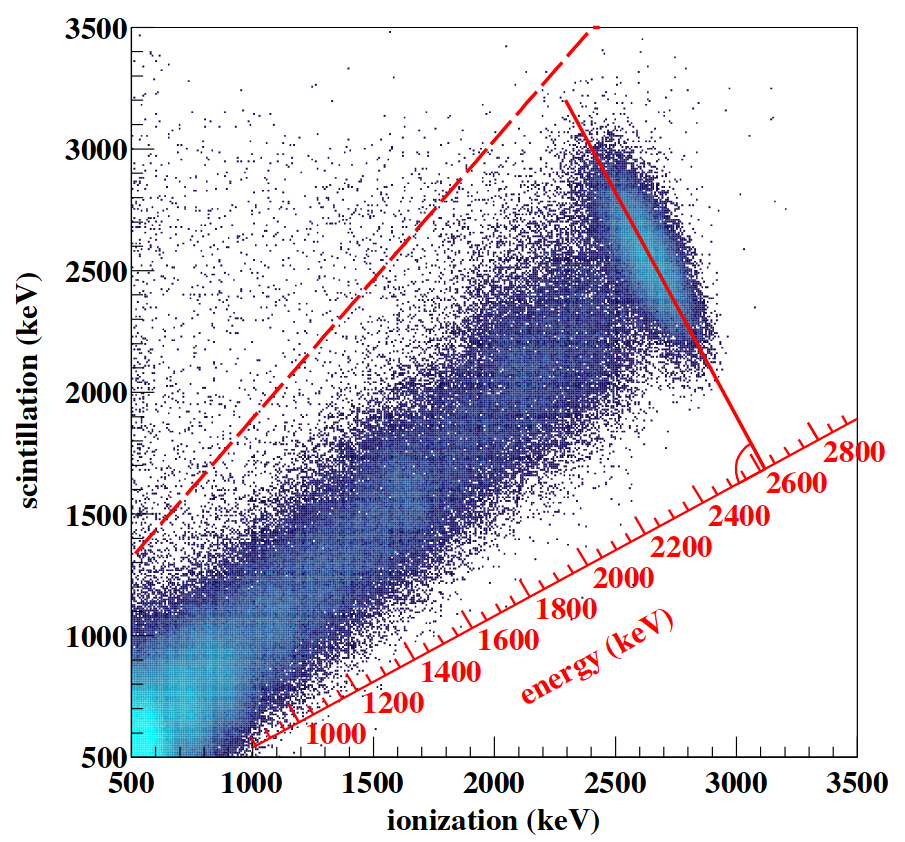
\includegraphics[width=8cm]{neutrinophysics/fig_neutrinophysics/ionisation-to-scintillation_EXO-200.png}
  \caption{\label{fig:ratio_EXO-200}}

\end{figure}

\begin{figure}
  \centering
  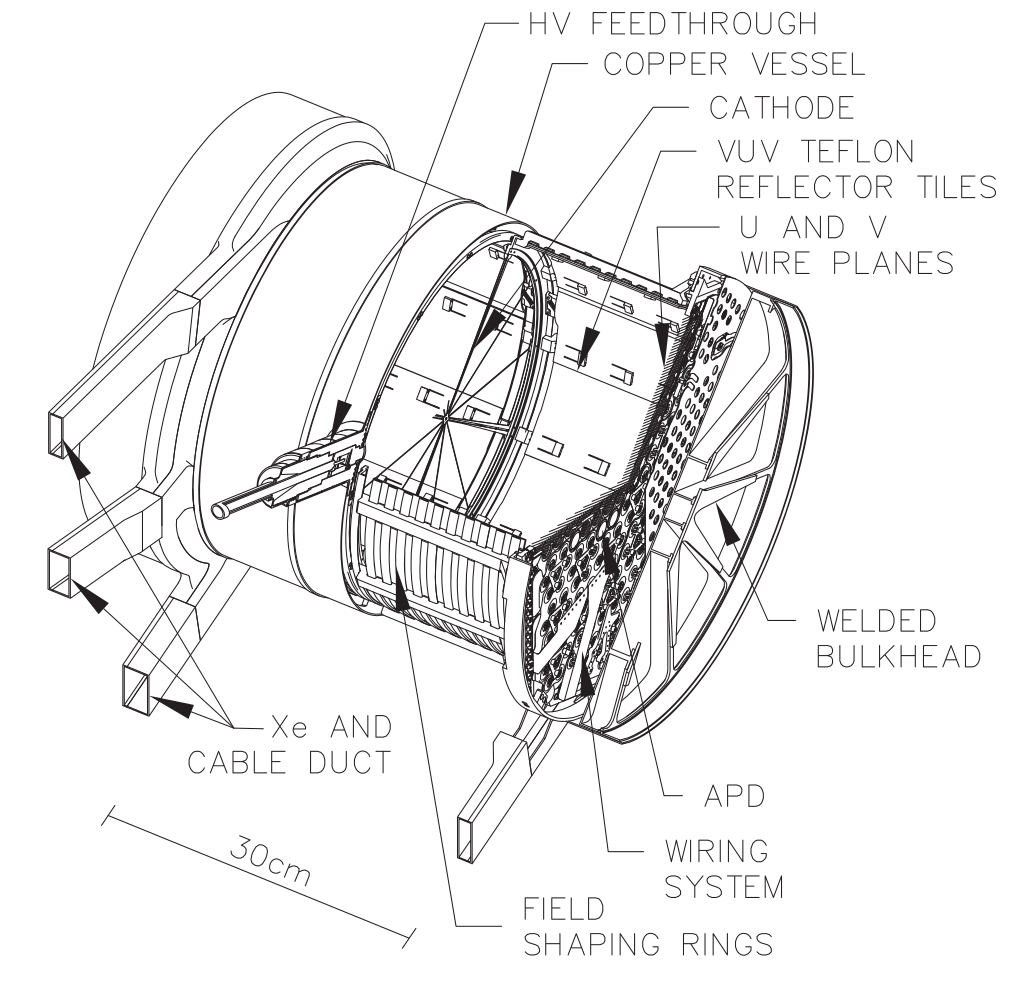
\includegraphics[width=8cm]{neutrinophysics/fig_neutrinophysics/EXO-200.png}
  \caption{\label{fig:EXO-200}}

\end{figure}

\paragraph{nEXO}
\paragraph{NEXT}
\paragraph{PandaX-III}
\subsection{Scintillators}
\label{subsec:scintillators}
\paragraph{KamLAND-ZEN and KamLAND2-ZEN}
\paragraph{ZICOS}
\paragraph{CANDLES}
\subsection{Tracking calorimeters}
\label{subsec:trackocalo}
Tracking calorimeters technology, instead of using a \emph{source-as-detector}, employ a passive source shaped as thin source foils of enriched $\beta\beta$ emitters.
Sources are placed at the detector centre, surrounded by two trackers allowing for particle identification (between electrons, positrons, $\gamma$ and $\alpha$ particles) and vertex reconstruction to improve the background rejection.
The whole is sandwiched between calorimeters enabling individual particle energy reconstruction.
In case of a discovery, this passive source tracking calorimeter technology provides topological information on angular emissions of the two electrons from $\beta\beta$ decay, making possible to distinguish between underlying mechanisms for $\zeronu$ decay.

\paragraph{SuperNEMO} experiment is a next-generation of detector, inheriting the lineage of the NEMO (Neutrino Ettore Majorana Observatory) experiments, which successfully studied multiple isotopes as enriched Molybdenum $^{100}$Mo.



\begin{center}
  \begin{table}
    \begin{tabular}{|l|c|c|c|c|}
      \hline
      Experiment & Isotope & M (kmol)&$\Tbeta$ ($90$ \% C.L.)&  $\mbb$ (meV)\\
      \hline \hline
      GERDA~\cite{art:GERDA2019}        & $^{76}Ge$  & $0.41$  & $9\times 10^{25}$          & $104-228$    \\
      MAJORANA~\cite{art:majorana2019}  & $^{76}$Ge  & $0.34$  & $2.7\times 10^{25}$        & $157-346$    \\
      CUPID-$0$~\cite{art:CUPID2018}    & $^{82}$Se  & $0.063$ & $0.24\times 10^{25}$       & $394-810$    \\
      CUORE~\cite{art:CUORE2018}        & $^{130}$Te & $1.59$  & $1.5\times 10^{25}$        & $162-757$    \\
      EXO-$200$~\cite{art:EXO2018}      & $^{136}$Xe & $1.04$  & $1.8\times 10^{25}$        & $93-287$     \\
      KamLAND-Zen~\cite{art:KamLAND2016}& $^{136}$Xe & $2.52$  & $10.7\times 10^{25}$       & $76-234$     \\
      \hline
    \end{tabular}
  \end{table}
\end{center}
